\documentclass[english]{article}
\usepackage{graphicx}
\usepackage[T1]{fontenc}
\usepackage[latin9]{inputenc}
\usepackage{amstext}
\usepackage{amsmath}
\usepackage{amsfonts}
\usepackage{amssymb}
\usepackage{babel}
\usepackage{courier}
\usepackage[margin=1in]{geometry}
\usepackage{graphicx}
\usepackage{caption}
\usepackage{subfigure}

\begin{document}

\title{Final Documentation: \\Matrix Product States for Probability Dynamics}


\author{Peter Gjeltema (gjeltema@princeton.edu)
	   \\ Peiqi Wang (peiqiw@princeton.edu)
	    \\ Jun Xiong (xiong@princeton.edu) 
	    \\ Bin Xu (binx@princeton.edu) 
	    \\ Liangsheng Zhang(liangshe@princeton.edu)}
	    
\date{\today}

\maketitle

\section{Introduction}

The matrix product state (MPS) is a novel numerical algorithm that is
widely used in quantum many-body physics. For a problem of quantum
spin chains, the states live in a Hilbert space expanded by the states
of each spin (referred to as ``orbitals'' hereafter), and the dimension
of that Hilbert space is $m^{N}$ for a chain of length $N$ where each orbital has $m$ choices. 
The dimension of the state space
grows exponentially with $N$, making it extremely hard to simulate
a system consisting of a few dozen sites. 

In 1995, White \cite{white} proposed
the density matrix renormalization group (DMRG), which proves to be an extremely efficient algorithm for one dimensional systems. Researchers of the next decade were aware of the ubiquitous relation between entanglement and dimensionality allowing the state to be approximated as the product of matrices \cite{schollwock}. Some recent developments include extension of the algorithm to higher dimensions\cite{cirac} and to critical systems\cite{vidal}.

This inter-departmental collaborative work applies this algorithm to other interesting problems. The algorithm's inherent probabilistic nature motivates its application to other difficult problems in probability theory and stochastic processes. An especially interesting example is the Markov process consisting of many degrees of freedom, which also forms an exponentially growing state space. 

We have developed  a generic MPS solver and compare results from some simple applications with that of exact transition matrix solutions. We start with a simple model of the dynamics of human relations (``Angry Boys" model), and move on to included other more sophisticated models. Due to the time limitation, this project focuses on one dimensional models for which the algorithm is well-established in physics. Higher dimensionality or highly correlated relationships offering the most realistic relevance will be left to future work.

\section{Background}

\subsection{The difficult many body problem}

When we have a state as a vector in the Hilbert space, it is expressed
as

\[
|\psi\rangle=\sum_{\{\sigma_{i}\}}A_{\{\sigma_{i}\}}|\sigma_{1}\sigma_{2}\sigma_{3}\cdot\cdot\cdot\sigma_{N}\rangle
\]
where $|\sigma_{1}\sigma_{2}\sigma_{3}\cdot\cdot\cdot\sigma_{N}\rangle$
is a product basis of the local Hilbert space on different sites.

Applying a linear time-evolution operator $\hat{O}$ on this state,
the general form of $\hat{O}$ is

\[
\hat{O}=\sum_{\{\sigma\},\{\sigma'\}}|\sigma'_{1}\sigma'_{2}\sigma'_{3}\cdot\cdot\cdot\sigma'_{N}\rangle\langle\sigma_{1}\sigma_{2}\sigma_{3}\cdot\cdot\cdot\sigma_{N}|O_{\{\sigma'\}\{\sigma\}}
\]
where $\langle\sigma_{1}\sigma_{2}\sigma_{3}\cdot\cdot\cdot\sigma_{N}|$ is a vector in the dual Hilbert space and $O_{\{\sigma'\}\{\sigma\}}$ is a complex number that represents the amplitude of transition. The application of this operator on the state is naturally written as
\[
\hat{O}|\psi\rangle=\sum_{\{\sigma\},\{\sigma'\}}|\sigma'_{1}\sigma'_{2}\sigma'_{3}\cdot\cdot\cdot\sigma'_{N}\rangle\langle\sigma_{1}\sigma_{2}\sigma_{3}\cdot\cdot\cdot\sigma_{N}|\ O_{\{\sigma'\}\{\sigma\}}\sum_{\{\sigma''_{i}\}}A_{\{\sigma_{''i}\}}|\sigma''_{1}\sigma''_{2}\sigma''_{3}\cdot\cdot\cdot\sigma''_{N}\rangle
\]
Using the orthonormal condition of basis, it can be simplified to

\[
\hat{O}|\psi\rangle=\sum_{\{\sigma_{i}\}\{\sigma'_{i}\}}A_{\{\sigma_{i}\}}O_{\{\sigma'\}\{\sigma\}}|\sigma'_{1}\sigma'_{2}\sigma'_{3}\cdot\cdot\cdot\sigma'_{N}\rangle
\]


Despite its simple form, the actual computation is very difficult since
the summation is conducted over $N$ indices of $\sigma_{i}$
simultaneously. Therefore, $m^{N}$ terms are computed. For the simplest case when
$m=2$ (only two elementary states for one site), $m^{N}\approx10^{9}$
for $N=30$, taking more than $10$ seconds for one single contraction.
The chain of $40$ sites is obviously intractable.


\subsection{Matrix Product States (MPS)}

To deal with the large number of terms in the contraction, we effectively split the space. Let's focus on the coefficient $A_{\{\sigma_{i}\}}=A_{\sigma_{1}\sigma_{2}\sigma_{3}\cdot\cdot\cdot\sigma_{N}}$.
From a direct point of view, it is a rank-N tensor which has N indices,
but we can group some indices so that it becomes $A_{\sigma_{1}(\sigma_{2}\sigma_{3}\cdot\cdot\cdot\sigma_{N})}$
with only $2$ indices where the first has $m$ possible values and
the second has $m^{N-1}$. Grouping $N-1$ indices means making a
bijection map from $N-1$ numbers varying between $1$ and $m$ to
a single integer varying from $1$ to $m^{N-1}$. This re-indicing
trick is crucial in MPS algorithms.

We then treat this bi-index object $A_{\sigma_{1}(\sigma_{2}\sigma_{3}\cdot\cdot\cdot\sigma_{N})}$
as a matrix with $\sigma_{1}$ the row index and $(\sigma_{2}\sigma_{3}\cdot\cdot\cdot\sigma_{N})$
the column index, thus forming a $m\times m^{N-1}$ matrix. Applying
singular value decomposition (SVD) on this matrix gives 
\[
A_{\sigma_{1}(\sigma_{2}\sigma_{3}\cdot\cdot\cdot\sigma_{N})}=U_{m_{1}}^{\sigma_{1}}S_{m_{1}m_{2}}V_{m_{2}(\sigma_{2}\sigma_{3}\cdot\cdot\cdot\sigma_{N})}=U_{m_{1}}^{\sigma_{1}}\tilde{V}_{m_{1}(\sigma_{2}\sigma_{3}\cdot\cdot\cdot\sigma_{N})}
\]
where $U$ is a $m\times m$ unitary matrix and $S$ is a $m\times m$
diagonal matrix with non-negative diagonal elements arranged in descending
order. We apply a similar procedure on $\tilde{V}_{m_{1}(\sigma_{2}\sigma_{3}\cdot\cdot\cdot\sigma_{N})}$
by re-arranging indices as $\tilde{V}_{m_{1}(\sigma_{2}\sigma_{3}\cdot\cdot\cdot\sigma_{N})}=\tilde{V}_{(m_{1}\sigma_{2})(\sigma_{3}\cdot\cdot\cdot\sigma_{N})}$
and applying a similar SVD:

\[
\tilde{V}_{(m_{1}\sigma_{2})(\sigma_{3}\cdot\cdot\cdot\sigma_{N})}=U_{(m_{1}\sigma_{2})m_{2}}S_{m_{2}m_{2}'}V_{m_{2}'(\sigma_{3}\cdot\cdot\cdot\sigma_{N})}=U_{m_{1}m_{2}}^{\sigma_{2}}\tilde{V}_{m_{2}(\sigma_{3}\cdot\cdot\cdot\sigma_{N})}
\]
where the second ``$=$'' reshapes the $U$ matrix and multiplied
the $S$ and $V$ matrices. 

Noticing that $\tilde{V}_{m_{2}(\sigma_{3}\cdot\cdot\cdot\sigma_{N})}$
is almost the same as $\tilde{V}_{m_{1}(\sigma_{2}\sigma_{3}\cdot\cdot\cdot\sigma_{N})}$
except for having one fewer $\sigma_{i}$, we apply this procedure
inductively and write the original coefficient tensor as

\[
A_{\{\sigma_{i}\}}=U_{m_{1}}^{\sigma_{1}}U_{m_{1}m_{2}}^{\sigma_{2}}U_{m_{2}m_{3}}^{\sigma_{3}}\cdot\cdot\cdot U_{m_{N-1}m_{N}}^{\sigma_{N}}
\]
This form is called the matrix product state, $\sigma_{i}$'s
are called ``physical indices', and $m_{i}$'s are called ``auxiliary
indices''. It is worth noting that, in general, operators can also
be decomposed in this way, although it is usually more convenient
to directly construct operators in matrix product form. This representation
is extremely convenient since each matrix $U$ contains only one physical
index, and the application of a matrix product linear operator
on a matrix product state only involves the contraction of a few indices.

To illustrate, if we have a linear operator $O_{\{\sigma'\}\{\sigma\}}=O_{n_{1}}^{\sigma'_{1}\sigma_{1}}O_{n_{1}n_{2}}^{\sigma'_{2}\sigma_{2}}O_{n_{2}n_{3}}^{\sigma'_{3}\sigma_{3}}\cdot\cdot\cdot O_{n_{N-1}n_{N}}^{\sigma'_{N}\sigma_{N}}$
then applying this operator on the MPS is actually the contraction
on $m$, $n$ and $\sigma_{i}$ space. The traditional way corresponds
to first contracting $m$ and $n$ spaces, and then $\sigma$. However, this
novel method contracts the $\sigma$ space first and then $m$ and
$n$. The specific order of contraction is:
\begin{itemize}
\item Compute $\sum_{\sigma_{i}}O_{n_{i-1}n_{i}}^{\sigma'_{i}\sigma_{i}}A_{m_{i-1}m_{i}}^{\sigma_{i}}=M_{n_{i-1}n_{i}m_{i-1}m_{i}}^{\sigma'_{i}}$
for all $i$'s
\item $\sum_{n_{1}m_{1}}M_{n_{1}m_{1}}^{\sigma'_{1}}M_{n_{1}n_{2}m_{1}m_{2}}^{\sigma'_{2}}=\tilde{M}_{n_{2}m_{2}}^{\sigma'_{1}\sigma'_{2}}$
\item $\sum_{n_{2}m_{2}}\tilde{M}{}_{n_{2}m_{2}}^{\sigma'_{1}\sigma'_{2}}M_{n_{2}n_{3}m_{2}m_{3}}^{\sigma'_{3}}=\tilde{M}_{n_{3}m_{3}}^{\sigma'_{1}\sigma'_{2}\sigma'_{3}}$
\item keep doing this, until we finish the multiplication of all these objects
and get $\tilde{M}^{\sigma'_{1}\sigma'_{2}\cdot\cdot\cdot\sigma'_{N}}=A_{\sigma'_{1}\sigma'_{2}\cdot\cdot\cdot\sigma'_{N}}$
which is the final result, coefficients of the new state $|\psi'\rangle=\sum_{\{\sigma'_{i}\}}A_{\sigma'_{1}\sigma'_{2}\cdot\cdot\cdot\sigma'_{N}}|\sigma_{1}\sigma_{2}\text{\ensuremath{\cdot}}\text{\ensuremath{\cdot}}\text{\ensuremath{\cdot}}\sigma_{N}\rangle$.
\end{itemize}

\subsection{Approximation}

It may seem unclear why our algorithm seems to transform a
 problem scaling exponentially to polynomial time; indeed, it should be.
We did not talk about the dimension of auxiliary space $m_{i}$ and
$n_{i}$, which should grow exponentially. The method is useful
only when the interaction is local or short-range, meaning the
degree of freedom on one site  effectively interacts only with some
of its neighbors. It is proven that in this case, the diagonal terms
in the $S$ matrix decay exponentially, effectively enabling a cut-off
in auxiliary space keeping only a finite number of $\chi$ dimensions. Thus, all $U$'s are at most $\chi\times\chi$ dimensional matrices.
$\chi$ is in this case called the bound dimension. The effectiveness of this algorithm
relies deeply on the fact that a large $\chi$ is unnecessary to achieving accurate
results. It is proven that in all 1-dimensional problems away from critical
points, $\chi$ does not grow with system size (the length); in critical
1-dimensional models, $\chi\propto N^{\lambda}$ (polynomial) and
in 2D, $\chi\propto\exp W$ which is the exponential of short dimension.


\subsection{Matrix Product Operators (MPO)}
The Hamiltonian in quantum mechanics, or equivalently the transitional matrix in stochastic processes, can be written as a series of matrix product operators where each matrix only applies on one site.
We considered four different models to implement our MPS algorithm.
\subsubsection{AngryBoys Model}
\begin{displaymath}
H = pI + (1-p)\sum_{i=1}^{n-1}\frac{1}{n-1}\sigma_i^x\otimes\sigma_{i+1}^x,
\end{displaymath}
where $I$ is a $2^n\times2^n$ identity matrix and 
\begin{displaymath}
\sigma_i^x = 
\begin{pmatrix}
0 & 1 \\
1 & 0
\end{pmatrix}
\end{displaymath}
As described in 3.1 Model.
The MPO of this model is 
$$
O=W^{[1]}W^{[2]} ... W^{[L]}
$$
And it can be encoded by the operator valued matrices below:
$$
W^{i}=
\begin{pmatrix}
I & 0 & 0 \\
S_x & 0 & 0 \\
0 & qS_x & I
\end{pmatrix}
$$
And  we have $W^1=\begin{pmatrix}p I & q S_x & I\end{pmatrix}$ on the first site of the chain, 
$$W^L=\begin{pmatrix}
I \\ S_x \\ 0
\end{pmatrix}$$
on the last site.

\subsubsection{RadiatingBoys Model}
\begin{displaymath}
H=p_0 I + p_1 \sum_{i=1}^{n-1}\frac{1}{n-1}\sigma_i^x\otimes\sigma_{i+1}^x + p_2 \sum_{i=1}^{n-2}\frac{1}{n-2}\sigma_i^x\otimes\sigma_{i+2}^x
\end{displaymath}
In this model, the state of a boy could be affected by both its nearest neighbor and its second nearest neighbor. And the MPO can be decomposed into the following matrices:
$$
W^{i}=
\begin{pmatrix}
I & 0 & 0 & 0 \\
S_x & 0 & 0 & 0 \\
0 & I & 0 & 0 \\
0 & p_1 S_x & p_2 S_x & I
\end{pmatrix}
$$
and $W^1=\begin{pmatrix}p_0 I & p_1 S_x & p_2 S_x & I\end{pmatrix}$ and 
$$W^L=
\begin{pmatrix}
I \\ S_x \\ 0 \\0
\end{pmatrix}$$


\subsubsection{Exponentialboys Model}
\begin{displaymath}
H = P (I + J \sum_{i=1}^{n-1} \sum_{j=i+1}^{n-1} K^{j-i}\sigma_i^x\otimes\sigma_j^x)
\end{displaymath}
The MPO of this model comprises of matrices:
$$W^{i}=
\begin{pmatrix}
I & 0 & 0 \\
S_x & K I & 0 \\
0 & J K S_x & I
\end{pmatrix}
$$,
$W^1=\begin{pmatrix}p_0 I & J K S_x & I\end{pmatrix}$ and 
$$W^L=
\begin{pmatrix}
I \\ S_x \\0
\end{pmatrix}$$.


\subsubsection{Projectionboys Model}
\begin{displaymath}
H = p_0 I +  \sum_{i=1}^{n-1}(\frac{p_1}{n-1}\sigma_i^x\otimes\sigma_{i+1}^x + \frac{q_1}{n-1}\pi_i^+\otimes\pi_{i+1}^- + \frac{q_2}{n-1}\pi_i^+\otimes\pi_{i+1}^-)
\end{displaymath}
The components of the MPO are:
$$W^{i}=
\begin{pmatrix}
I & 0 & 0 & 0 & 0 \\
S_x & 0 & 0  & 0 & 0 \\
\pi_i^+ & 0 & 0  & 0 & 0 \\
\pi_i^- & 0 & 0  & 0 & 0 \\
0 & p_1 S_x & q_1 \pi_i^+  & q_2 \pi_i^- & I
\end{pmatrix}$$,
$W^1=\begin{pmatrix}p_0 I & p_1 S_x & q_1 \pi_i^+ & q_2 \pi_i^- & I\end{pmatrix}$ and
$$W^L=
\begin{pmatrix}
I \\ S_x \\ \pi_i^+ \\ \pi_i^- \\ 0
\end{pmatrix}$$.

\section{Program Overview}
In this project, we extend the usage of MPS and MPO to problems concerning stochastic processes. Particularly, we  consider the time evolution of a probability distribution expressed in a vector form, where the dynamics are specified by a probability transition matrix.

\begin{figure}[htbp]
\begin{center}
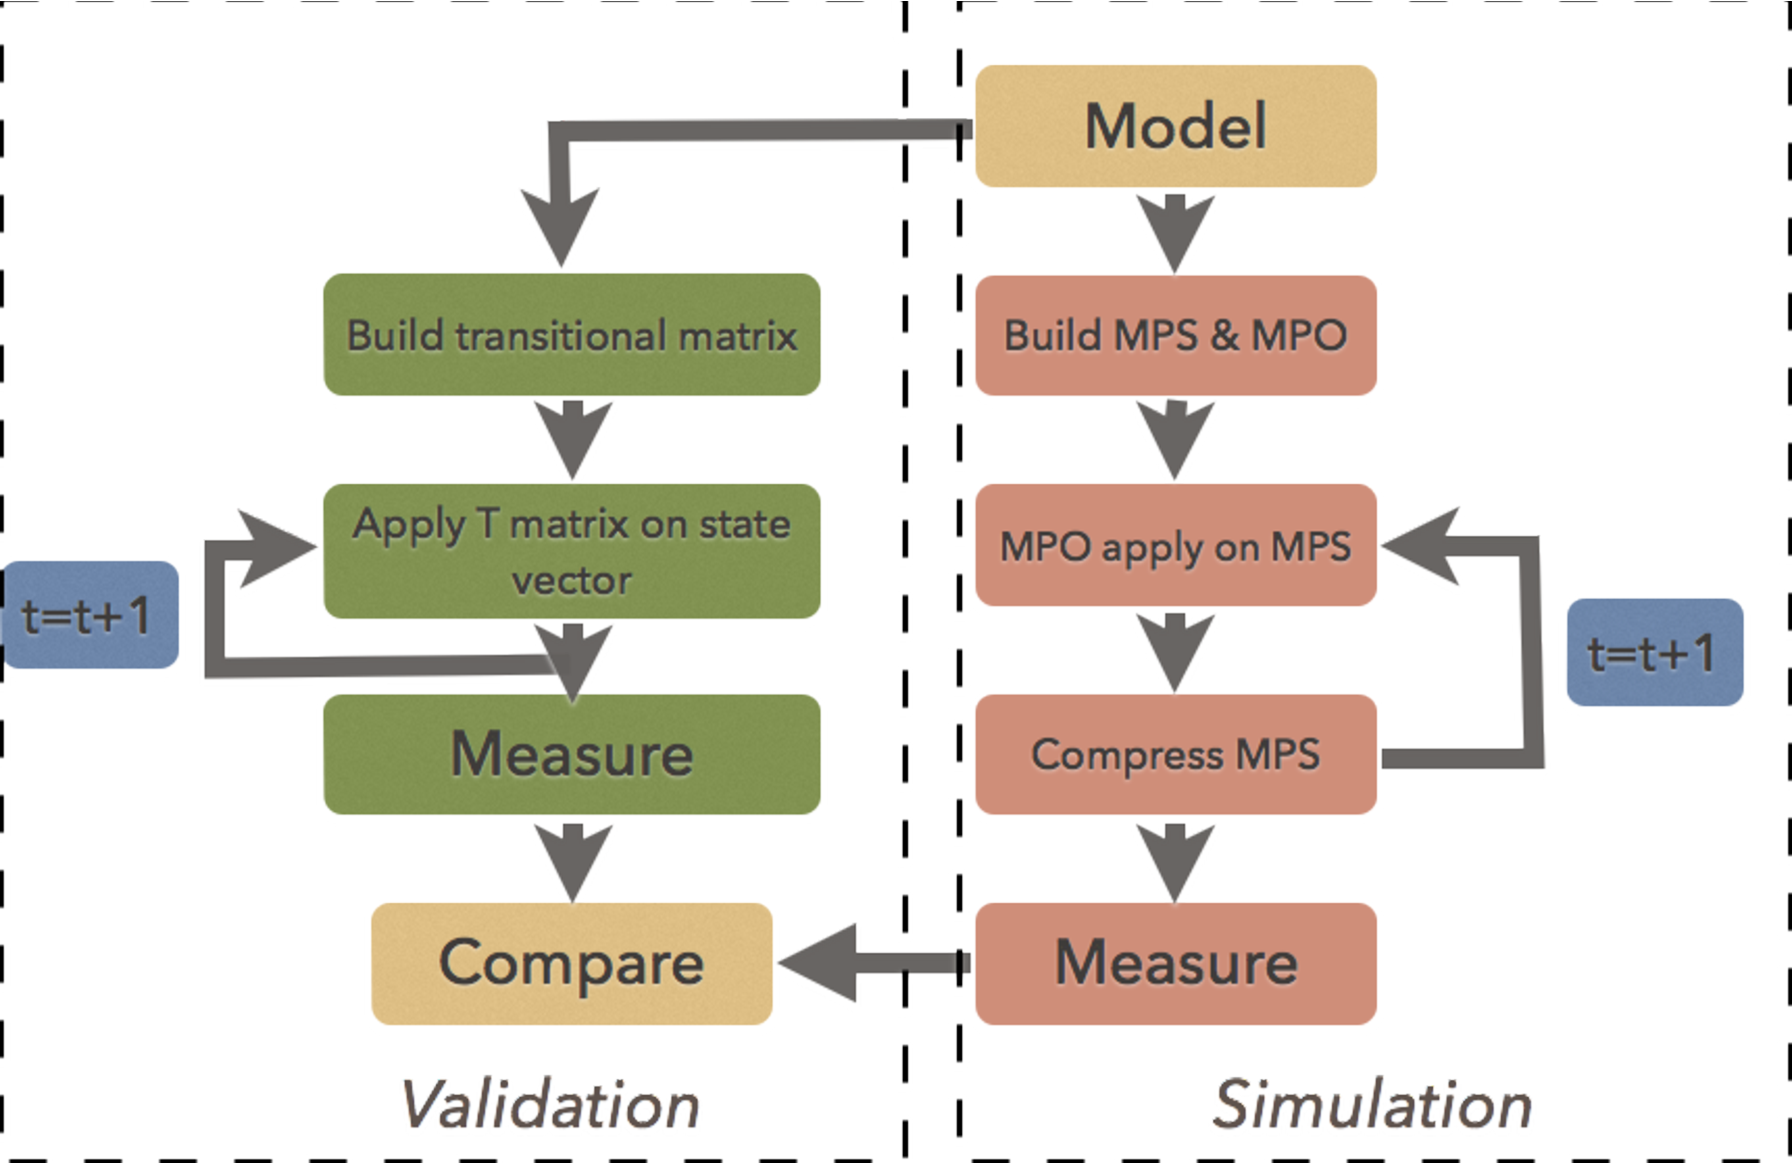
\includegraphics[width=0.7\textwidth]{flow_chart_new.pdf}
\caption{The flow chart of our program.}
\label{fig:flow_chart}
\end{center}
\end{figure}

\begin{figure}[htbp]
\begin{center}
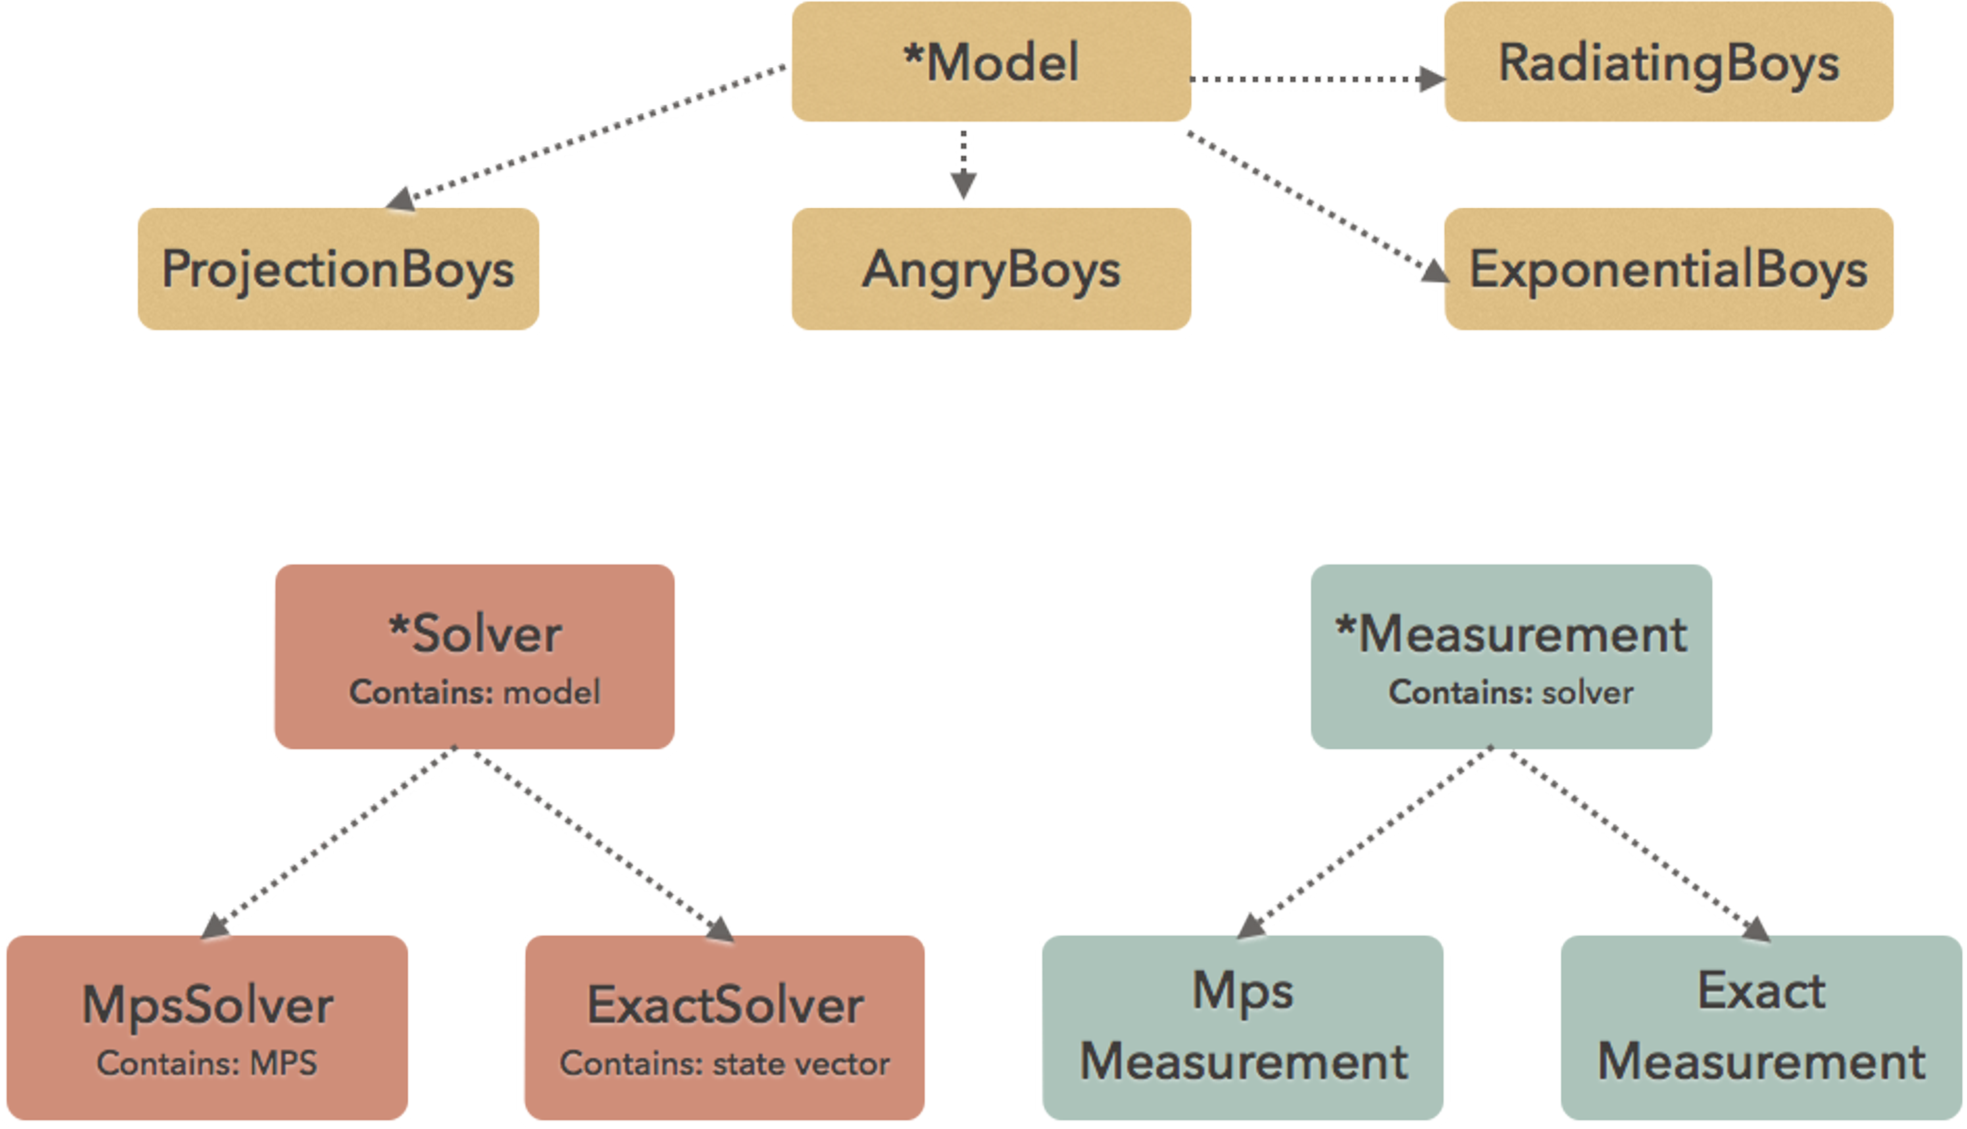
\includegraphics[width=0.7\textwidth]{class_diagram_new.pdf}
\caption{A bird view of our classes.}
\label{fig:class_diagram}
\end{center}
\end{figure}


The implementation is summarized in Fig.~\ref{fig:flow_chart}. The model is implemented in multiple ways. The classes used are described in Fig.~\ref{fig:class_diagram}.

\subsection{Exact Solution}

\subsubsection{Solving the Problem in Theory}
	The many body problem is treated one dimensionally, with $n$ agents on a line at positions $i=1,2,\cdots,n$. Each body can occupy one of two states $(1,0)^T$ and $(0,1)^T$, corresponding to a state space of size $2^n$. The dynamics of the system at each time step can be represented by the following probability transition matrix:
\begin{displaymath}
H = pI + (1-p)\sum_{i=1}^{n-1}\frac{1}{n-1}\sigma_i^x\otimes\sigma_{i+1}^x,
\end{displaymath}
where $I$ is a $2^n\times2^n$ identity matrix and
\begin{displaymath}
\sigma_i^x =
\begin{pmatrix}
0 & 1 \\
1 & 0
\end{pmatrix}
\end{displaymath}
operates on the state space of position $i$.  Qualitatively, the transition matrix models the system by capturing interactions between neighboring bodies. A body's state remains constant with probability $p$, and flips its state with probability  $(1-p)/(N-1)$. Consider the $Angry Boys$ model as an example: the system is an abstraction of boys standing in a line, and their mood is in a state of either  "anger" $(1,0)^T$ or "tranquility" $(0,1)^T$. Their respective states are in turn influenced by their left and right neighbors.

\subsubsection{Solving the Problem Computationally}
	Simulating a solution to the many body problem is computationally intense. Construction of the transition matrix at each time step requires a summation over $N$ indices of $\sigma_{i}$
simultaneously, meaning $m^{N}$ terms are examined. For a simply model where a body occupies one of two elemetary states, $m^{N}\approx10^{9}$ for $N=30$. A simulation of $40$ sites is impossible.  Nonetheless, an exact solution class $ExactSolver$ bounded by reasonably-sized state spaces has been constructed as a corroboration of results obtained through the MPS algorithm.

The $ExactSolver$ class takes the $Solver$ class as its parent. Its dependencies include the $numpy$ library, the deepcopy function of the $copy$ library, and a $Boys$ model from its respective parent class. Three functions defined in the class - $interpreter$, $step$, and $evolve$ - conduct simulation. Data from the simulation is collected in the form of lists. One list saves the state of the model at each time step, and one list saves the sum of probabilities at each step to ensure proper normalization of the model (probability cannot exceed 1).

The $interpreter$ function accepts the imported model, reads its information, and initiates the simulation. The model's information consists of the beginning transition matrix and the initial state. Once the transition matrix is set, and the initial state is set and saved, simulation can commence. This represents a change from the alpha version; orginally, $interpreter$ itself was used to initiate the transition matrix and initial state. The beta version now offers functions to do this so that models with more diverse properties can interact with the solver. For instance, models reflecting influence from only a left or right neighbor can direct their unique transition matrix to $ExactSolver$. Additional control over initial state conditions is also given.

The $step$ function is very simple. It first increments simulation time, and then produces a new state by calculating the tensor dot product of the transition matrix and previous state.

The $evolve$ function controls the flow of the simulation by taking as its argument the total number of time steps desired for the simulation. $evolve$ calls $step$ to produce a new state, and then appends this state and its norm to its respective data list. This process is done iteratively for the number of time steps, producing a time evolution of the model. 



\subsection{MPS class}
Parallel to the class \texttt{Exact}, we construct a class named \texttt{MPS} to store the MPS representation of the current state, to hold the MPO representation of the dynamics of the system and to comprise several functions necessary to updating the current state. The \texttt{MPS} class includes the following:
\\[3mm]
\noindent\textbf{Member data} We have the current state saved under a variable named \texttt{MPState}, which is a 3-d array storing $M^{\sigma_i}_{a_{i-1},a_i}$. The operator $O^{\sigma_i, \sigma'_i}_{n_{i-1}, n_i}$ is stored in a variable named \texttt{MPO}, which is a 4-d array. In addition, we store the time of the system in the variable \texttt{T}.
\\[3mm]
\noindent\textbf{Constructor} The constructor takes a model of type \texttt{Model} and an initial state as argument and initilize the members \texttt{MPState}, \texttt{MPO} and \texttt{T}. We  focus on using this to solve a handful of certain well-defined models.
\\[3mm]
\noindent\textbf{Methods} As is shown in the flow chart, to update the state from time $t$ to $t+1$, one must first apply the MPO to the MPS and then compress the state. The compression step is necessary because after applying MPO to MPS, the resulting MPS will have a  auxiliary space with greater degrees of freedom. The compression step consists of projecting the resulting MPS (which is of higher dimension) back to the initial space (of a lower dimension). We write the routine \texttt{Step} responsible for applying MPO and updating the current state \texttt{MPState}. This routine calsl \texttt{Compression} to make sure that the new state has the desired degrees of freedom.
Both \texttt{Step} and \texttt{Compression} will involve some basic operations of multiplication of arrays and summing over a certain number of indices (similar to matrix multiplication). We implement these basic operations so \texttt{Step} and \texttt{Compression} can call these routines.
Note that if we would to calculate the expectation of a physical quatity, or the marginal probability of a physical states, we have to do the "overlapping" operation of two MPS's. This again involves a number of basic operations defined in the class \texttt{MPS}. So, the members in the class \texttt{Measurement} conducting evaluation of expectations and probabilities is able to call the routines in the class \texttt{MPS}.
\\[3mm]
The \texttt{Compression} function of MPS will work iteratively. To initialize for the compression, we apply SVD to the MPS representation of the states, and then truncate the decomposed matrices with $\chi$ largest single values retained. The following steps of compression minimize $||\psi^i-\psi^{i-1} ||^{2}$ iteratively, where $\psi^{i-1}$ is the state from the previous step while $\psi^i$ is the state obtained for the new $ith$ step. The extrema condition in minimizing $||\psi^i-\psi^{i-1} ||^{2}$ require solving linear equations to get the new coefficients in the new matrices of the $ith$ step. After that the new state is normalized.
\\[3mm]

\subsection{Measurement Class}

The \texttt{Measurement} class includes functions for calculating the expectation of a given operator, the conditional probability of certain states, and possibly the correlation functions of different time steps. Both the conditional probability and correlation function may require us to store the MPS at each step. By calling this storage, we don't need to rerun the MPS procedure to calculate new physical quantities. And this is one of the advantages of MPS over Monte Carlo method. In the simplest form, the user can specify a set of states/operators through a defined structure, which are then combined with final state of the system to give (conditional) probabilities. If time permitted, we will try to extend the measurement to include time-dependent information.

\vspace{3mm}

\section{Implementation details}
\subsection{Compression by variation}
\subsubsection{Some maths}
Denote $|\psi\rangle=\sum_{\sigma}M^{\sigma_1}\dots M^{\sigma_L}$ the MPS to be compressed. The method of compression by variation consists of finding a new MPS $|\bar\psi\rangle=\sum_{\sigma}\bar M^{\sigma_1}\dots 
 \bar M^{\sigma_L}$ where each $\bar M^{\sigma_i}$ of desired size, such that the $L^2-$ distance between $|\bar\psi\rangle$ and $|\psi\rangle$ is minimized. Formally:
 \[
|\bar\psi\rangle = \arg\min_{|\phi\rangle=\sum_{\sigma}\bar M^{\sigma_1}\dots 
 \bar M^{\sigma_L}, M^{\sigma_L} \in \mathbb{R}^{d\times d} }\||\phi \rangle-|\psi\rangle\|^2
 \]
 This is a rather complicated optimization problem. One heuristic to tackle it involves iterative optimization. We start with an initial guess of the minimizer. We keep all other matrices fixed and minimize $\||\phi \rangle-|\bar\phi\rangle\|^2$ with respect to the matrix of the first physical site $\bar M^{\sigma_1}$. Upon obtaining the minimizer we update $|\bar\phi\rangle$, move to the next site and repeat this procedure. We do this until we reach the last physical site. This is called a sweep. We then repeat the sweep through the chain and check the $L^2-$ distance between original and compressed MPS after each sweep. We stop the process when $L^2-$ distance stops to decrease with respect to a user-defined level of tolerance.

The key in this algorithm is to minimize $\||\phi \rangle-|\bar\phi\rangle\|^2$ with respect to the matrix of a given physical site. This can be done by exploiting the first-order condition. Let us denote $M^*$ as the conjugate transpose of matrix $M$. Then at the optimum, for each $\sigma_i$ (physical states), $a_i$ and $a_{i-1}$ (auxiliary states), we must have
\[
0=\frac{\partial}{\partial M^{\sigma_i,*}_{a_i,a_{i-1}}} \||\phi \rangle-|\bar\phi\rangle\|^2 = \frac{\partial}{\partial M^{\sigma_i,*}_{a_i,a_{i-1}}} \left(-\langle\bar\psi | \psi\rangle +  \langle\bar\psi |\bar \psi\rangle \right)
\]
The last equality is due to the fact that $M^{\sigma_i,*}_{a_i,a_{i-1}}$ only shows up in $\langle\bar\psi|$. Further expansion of the equation provides that
\[
\begin{array}{rl}
0=&\displaystyle\frac{\partial}{\partial M^{\sigma_i,*}_{a_i,a_{i-1}}} \left(-\langle\bar\psi | \psi\rangle +  \langle\bar\psi |\bar \psi\rangle \right)\\\\
=&\displaystyle \sum_{\sigma\setminus\sigma_i}(\bar M^{\sigma_1,*}\dots\bar M^{\sigma_{i-1},*})_{1,a_{i-1}}(\bar M^{\sigma_{i+1},*}\dots\bar M^{\sigma_{L},*})_{a_{i},1}\bar M^{\sigma_1}\dots \bar M^{\sigma_i}\dots\bar M^{\sigma_L}\\\\
&-\displaystyle \sum_{\sigma\setminus\sigma_i}(\bar M^{\sigma_1,*}\dots\bar M^{\sigma_{i-1},*})_{1,a_{i-1}}(\bar M^{\sigma_{i+1},*}\dots\bar M^{\sigma_{L},*})_{a_{i},1} M^{\sigma_1}\dots  M^{\sigma_i}\dots M^{\sigma_L}
\end{array}
\]
Here $\sigma\setminus\sigma_i$ means the sum takes over all the physical sites except the $i-$th physical site. The above can be further simplified if we assume that $\bar M$ is under mixed-canonical form, i.e. $\sum_{\sigma_i}M^{\sigma_j,*}M^{\sigma_i}=Id, \forall j=1\dots i-1$ and $\sum_{\sigma_i}M^{\sigma_j}M^{\sigma_i,*}=Id, \forall j=i+1\dots L$. Under this assumption, the first term on the right hand side simplifies to $\bar M^{\sigma_i}_{a_{i-1},a_1}$, which is exactly the coefficient we are looking for. Then the equation can be written as
\[
\bar M^{\sigma_i}_{a_{i-1},a_1}=\sum_{a'_{i-1}a'_i}L_{a_{i-1},a'_{i-1}}M^{\sigma_i}_{a'_{i-1},a'_i}R_{a_i,a'_i}
\]
where $L$ is the overlap of $M$ and $\bar M$ from left to the $(i-1)$th state, and $R$ is the overlap of $M$ and $\bar M$ from right to the $(i+1)$th state. We call objects like $L$ and $R$ respectively the left partial overlap and the right partial overlap. Obviously from what has been described about the algorithm, the partial overlaps need to be used and updated during the sweeps. When implementing the algorithm, we store them in the lists \texttt{self.partial\textunderscore overlap\textunderscore lr} and \texttt{self.partial\textunderscore overlap\textunderscore rl}. Note that the last element of \texttt{self.partial\textunderscore overlap\textunderscore lr} and the first element of \texttt{self.partial\textunderscore overlap\textunderscore lr} are actually the full overlap of the compressed state and the original state. This is useful in computing the $L^2-$distance and in deciding when to stop the sweep.

Attention must also be paid to the normalization. Indeed, all the MPS studied here represent a probability distribution. Thus, summing over all the physical states must yield unity. However, this can no longer be guaranteed after the procedure of compression . Therefore, the result of compression must be normalized by its $L^1-$norm.

\subsubsection{Implementation}
The main routine for compression by variation is \texttt{self.compressionVariational}. It does the following operations:
\begin{itemize}
\item \texttt{self.initializeMpscVar}: Form a initial guess of the compressed MPS of desired size. It is then left or right canonized, depending on the direction of the first sweep. $L^2-$distance with the original MPS is calculated. 
\item \texttt{self.initializePartialOvl}: Initialize the partial overlap lists. Note that if the first sweep is from left to right, then we only have to initialize the right partial overlaps.
\item \texttt{self.compressionSweepLeftRight}: Perform a sweep from left to right. For each site, we calculate the matrix using left and right partial overlap. Before moving to the next site on the right, we have to left-normalize the current site (to preserve the mixed-canonical form) and update the left partial overlap list. At the end of the sweep, we calculate the $L^2-$distance with the original MPS and store the value in \texttt{self.cpr\textunderscore err}.
\item \texttt{self.compressionSweepRightLeft}: Perform a sweep from right to left. The idea is the same as described above.
\item We start the sweep with direction specified by the user and alternate the left and right sweeps until the $L^2-$distance recorded by \texttt{self.cpr\textunderscore err} converges.
\end{itemize}
Throughout the sweeps, we also keep track of the $L^1-$norm of the MPS. The User can choose whether to normalize the MPS after each sweep or after the completin of all sweeps.

\subsubsection{Usage}
\texttt{self.compressionVariational(direction,sweep\textunderscore nbr,norm)} compresses the MPS stored in \texttt{self.mps} and writes the results in \texttt{self.mpsc}. The User can set the dimension of compressed MPS via the variable \texttt{self.bound\textunderscore dimension}. The tolerance of convergence for sweeps can be accessed by \texttt{self.epsil}.  Options available for \texttt{self.compressionVariational} include:
\begin{itemize}
\item \texttt{direction}: the direction of first sweep. $0$ for left to right and $1$ for right to left. The default is to sweep from left to right first.
\item \texttt{sweep\textunderscore nbr}: The total number of sweeps the user desires to make. If  \texttt{sweep\textunderscore nbr}$ =0$, then sweeps will continue until convergence.
\item \texttt{norm}: whether to normalize after each sweep or after all the sweeps. If \texttt{norm} $=0$, the compressed MPS will be normalized after all the sweeps. If \texttt{norm} $=1$, the compressed MPS will be normalized after each sweep.
\end{itemize}
Example: \texttt{self.compressionVariational(, 4, 1)} will perform 4 compression sweeps, with the first one starting from right to left. The compressed MPS will be normalized after each sweep.

\section{Results}
\subsection{AngryBoys Model}
    Fig.\ref{fig:Angry_result} describes the main data that we obtained through the MPS method. The Angryboys Model was used. Fig.\ref{fig:Angry_result}a is the comparison between the compressed MPS method and the exact MPS method when the chain size $L=10$ and the bound dimension $\chi=10$. We calculated time evolution of the joint probability, the mean value, and the variance to find that the compressed MPS method agrees well with the exact method. Furthermore, in this model, all three quantities reach a limit at large enough time, indicating that this model is an aperiodic Markov chain. In Fig.\ref{fig:Angry_result}a, we examined the square error sum of the joint probability between the compressed MPS method and exact method at different bound dimension $\chi$. The figure clearly shows that the error decreases almost exponentially with the increasing bound dimension; and when the bound dimension is close or above 10, the error can be neglected for short chains. This confirms that our approximation is valid. Fig.\ref{fig:Angry_result}c gives the result for a long chain, where $L=100$ and $\chi=10$. Such a long chain case cannot be computed by the exact method since the size of the matrix grows exponentially with chain length. However with our compressed method, we can calculate the physical properties of this long chain in a short time. Here we only use a small bound dimension $\chi=10$ and the size of the matrix is not very large. Thus the MPS method has greatly reduced the computation load in this problem. And the result also reaches an equilibrium state. Fig.\ref{fig:Angry_result}d compares the time evolution of the joint probability of MPS method when the bound dimension $\chi$ is 10 and 20 respectively. At early time, the two bound dimensions will generate slightly different physical quantities, but in the long run, the two cases will converge. Such a converging behavior shows that a bound dimension around 10 can already provide a good approximation of a long chain in Angryboys Model. It indicates that our compressed matrices can simulate the exact result well in the long run, although the matrices have been truncated a great deal. However, we must admit that when the chain size grows larger than 200, the code has some errors and interruptions.
    
\begin{figure}[htbp]
\centering
\subfigure[Exact Model(Short Chain)]{
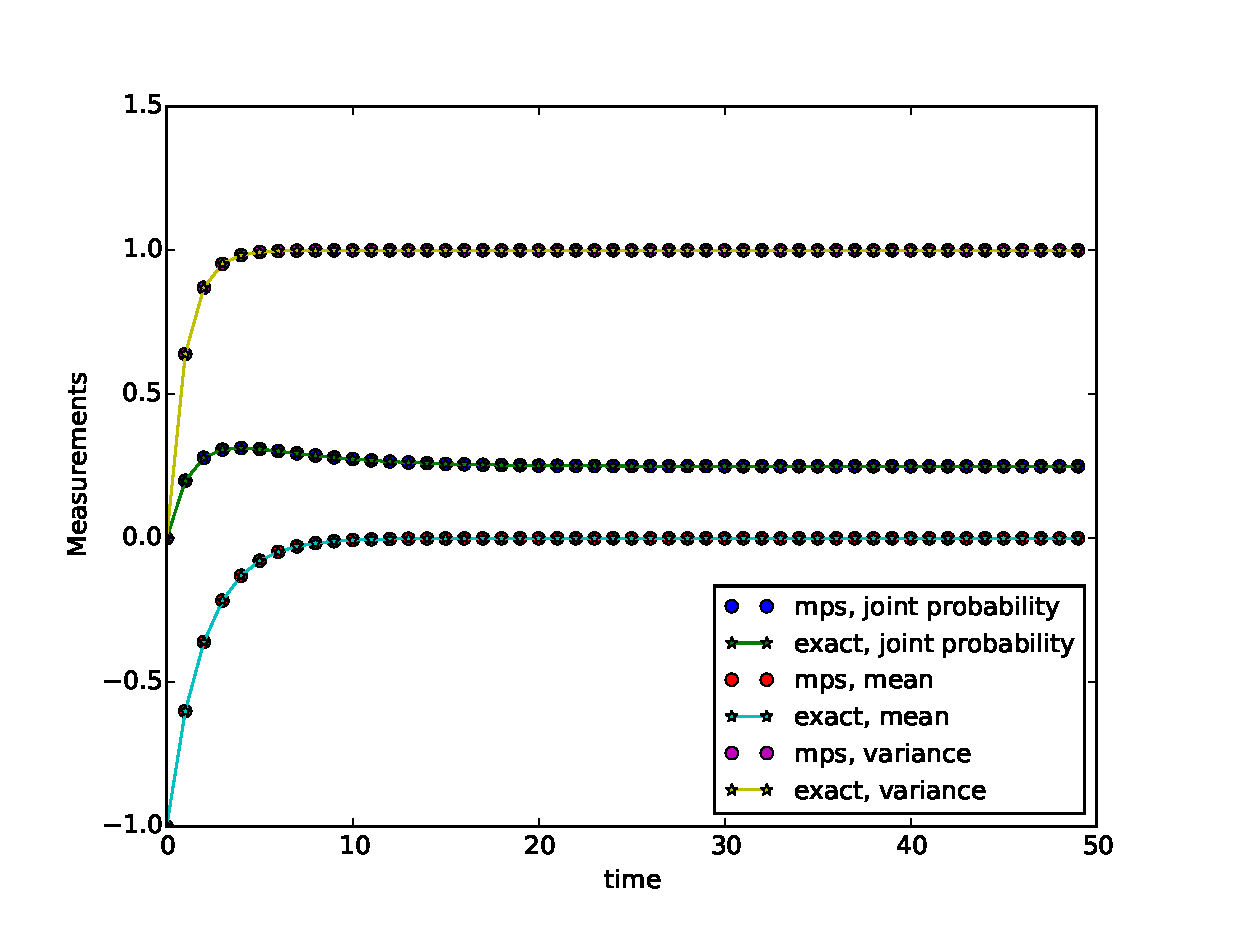
\includegraphics[scale=0.4]{Result_Fig/Angry_Exact_t50_s10_bd10.eps}}\hfill
\subfigure[Error with Different Bound Dimension]{
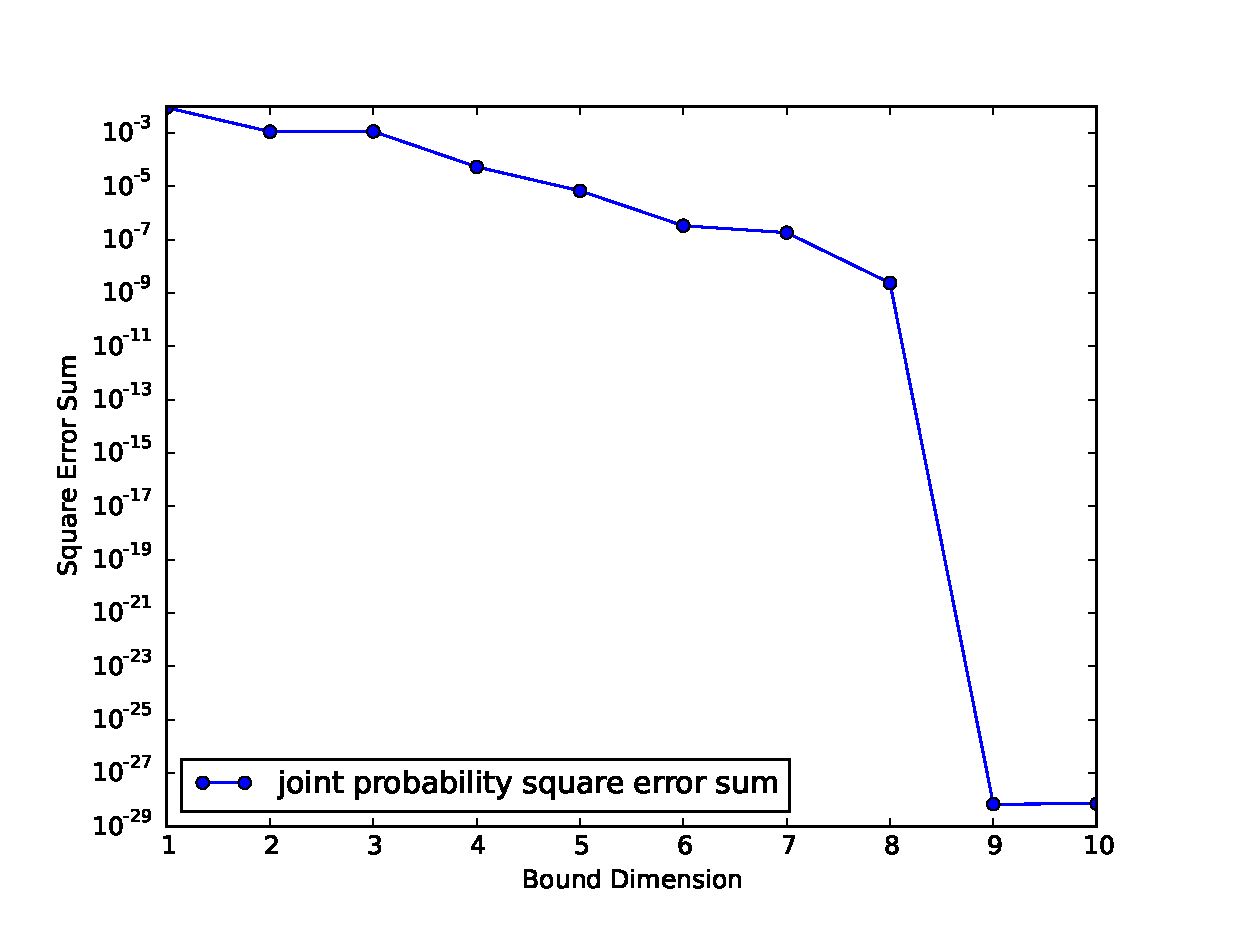
\includegraphics[scale=0.4]{Result_Fig/Angry_Error_t100_s10_bd10_log.eps}}
\subfigure[MPS long chain]{
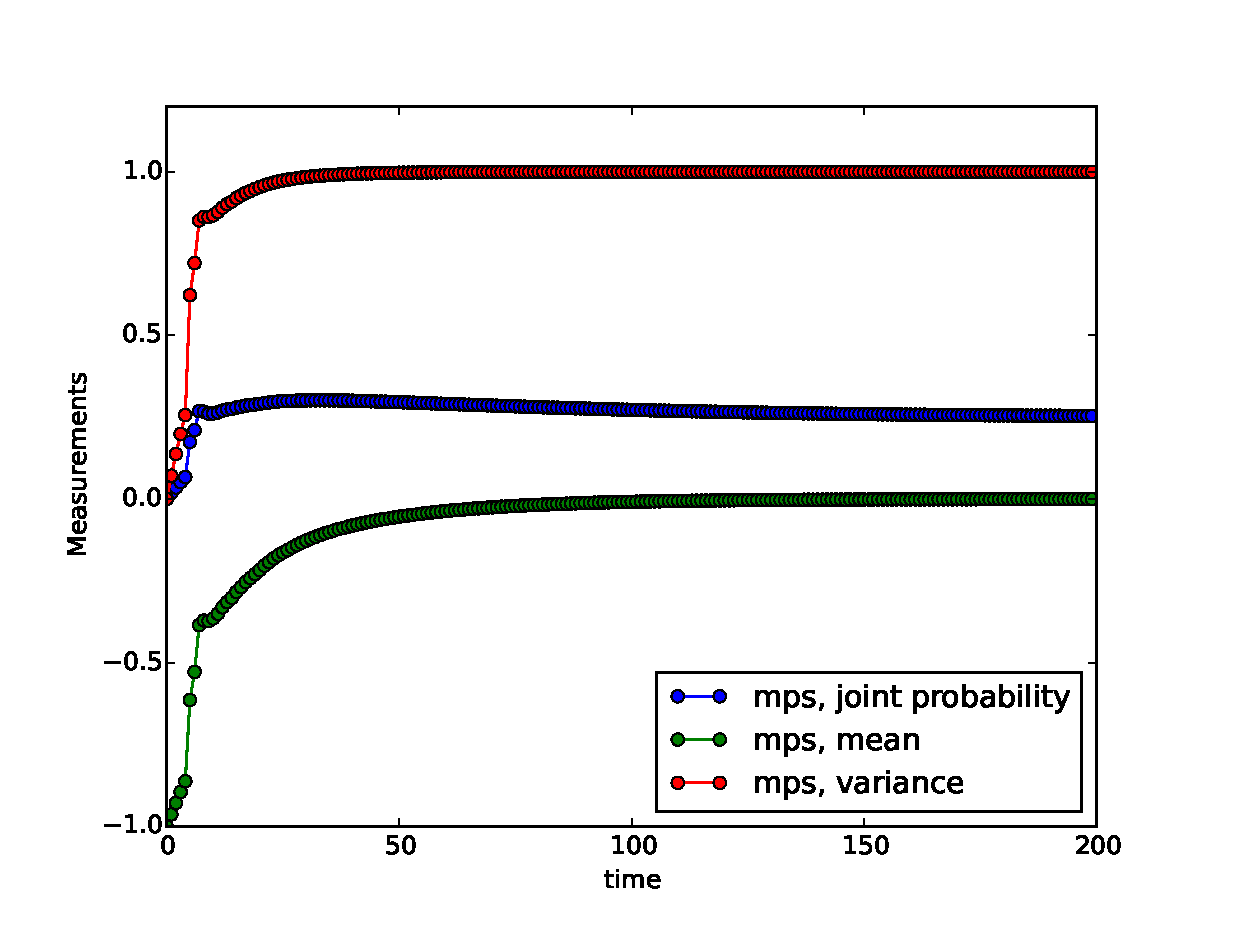
\includegraphics[scale=0.4]{Result_Fig/Angry_MPS_t200_s100_bd10.eps}}\hfill
\subfigure[MPS with Different Bound Dimension]{
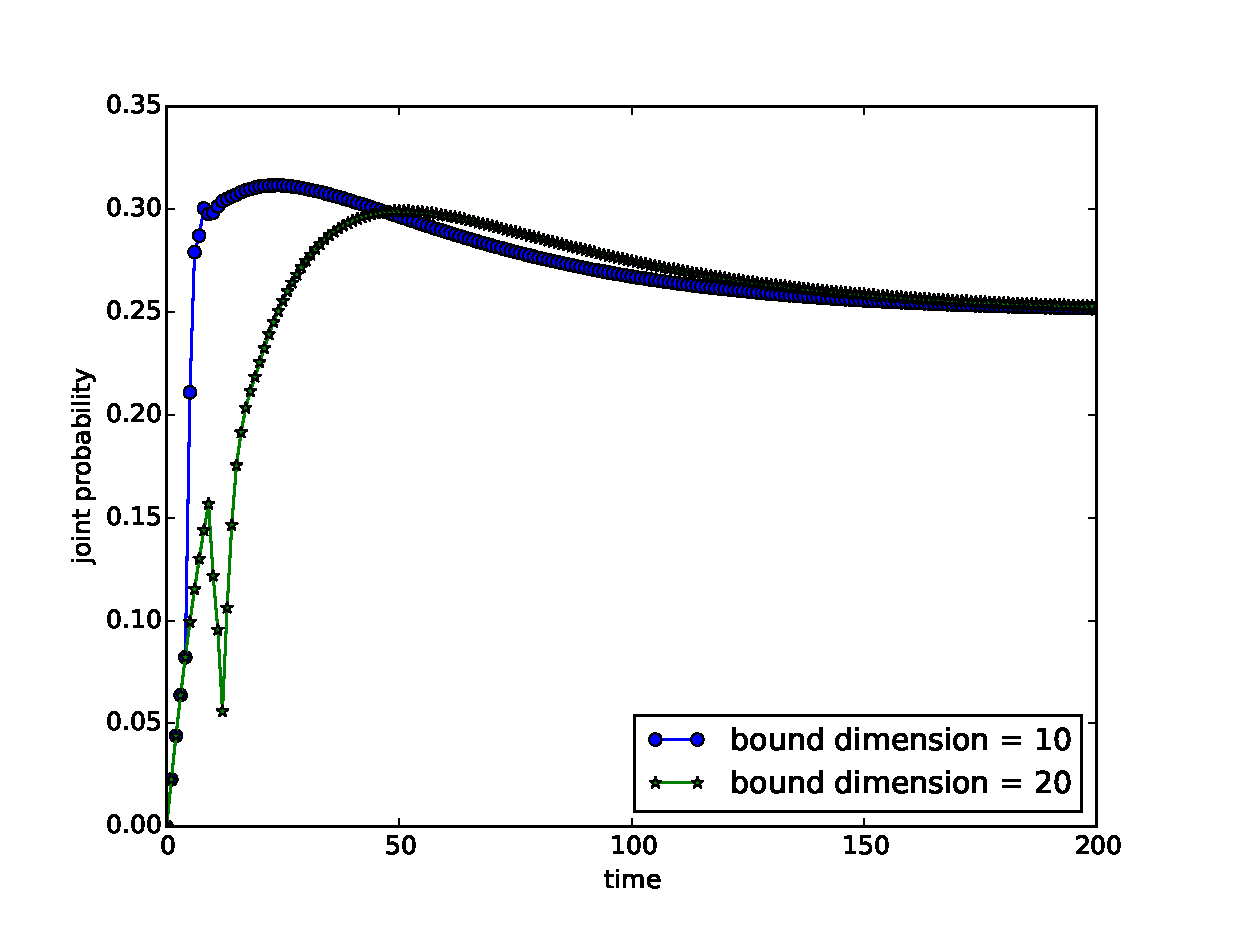
\includegraphics[scale=0.4]{Result_Fig/Angry_MPS_t200_s80_bd10to20.eps}}
  % \end{minipage}\\[1em]
  \caption{Results of Angry Boys Model.(a) gives the comparison of the joint probability, the mean value, and the variance between the MPS method and exact method. The chain size is 10, and the bound dimension $\chi$ is 10 in the MPS method. (b) shows the decay of square error sum with increasing bound dimensions. The error is computed between the approximation and exact method with a fixed time step of 100. (c) is the result of MPS method on a long chain with the size $L=100$. (d) compares the joint probability of the MPS method with two bound dimensions. The two curves converge in the long run.}
  \label{fig:Angry_result}
\end{figure}

\subsection{RadiatingBoys Model}
Fig.\ref{fig:Radiating_result} is the result of the Radiating Boys Model. 
\begin{figure}[htbp]
\centering
\subfigure[Exact Model(Short Chain)]{
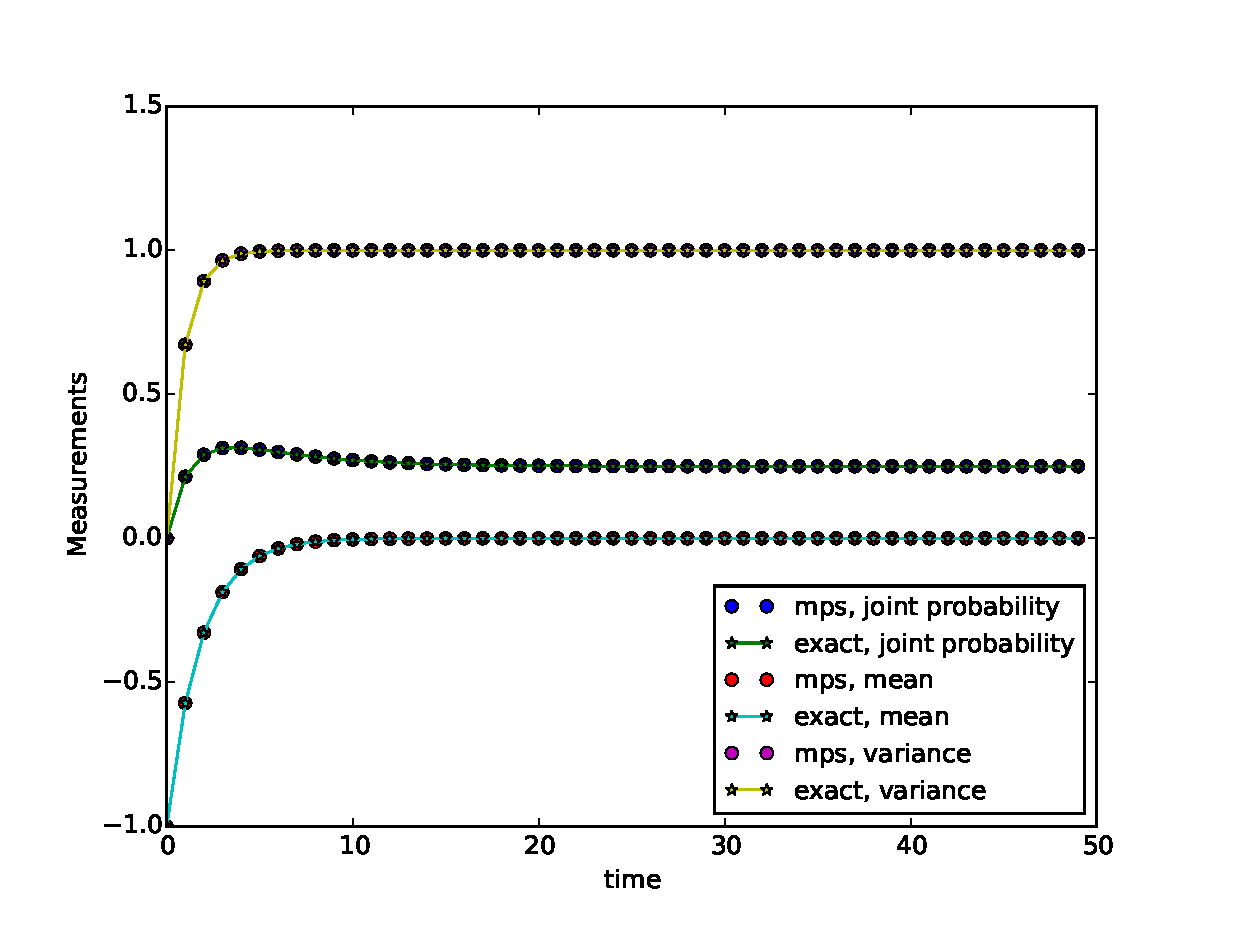
\includegraphics[scale=0.4]{Result_Fig/Radiating_Exact_t50_s10_bd10.eps}}\hfill
\subfigure[Error with Different Bound Dimension]{
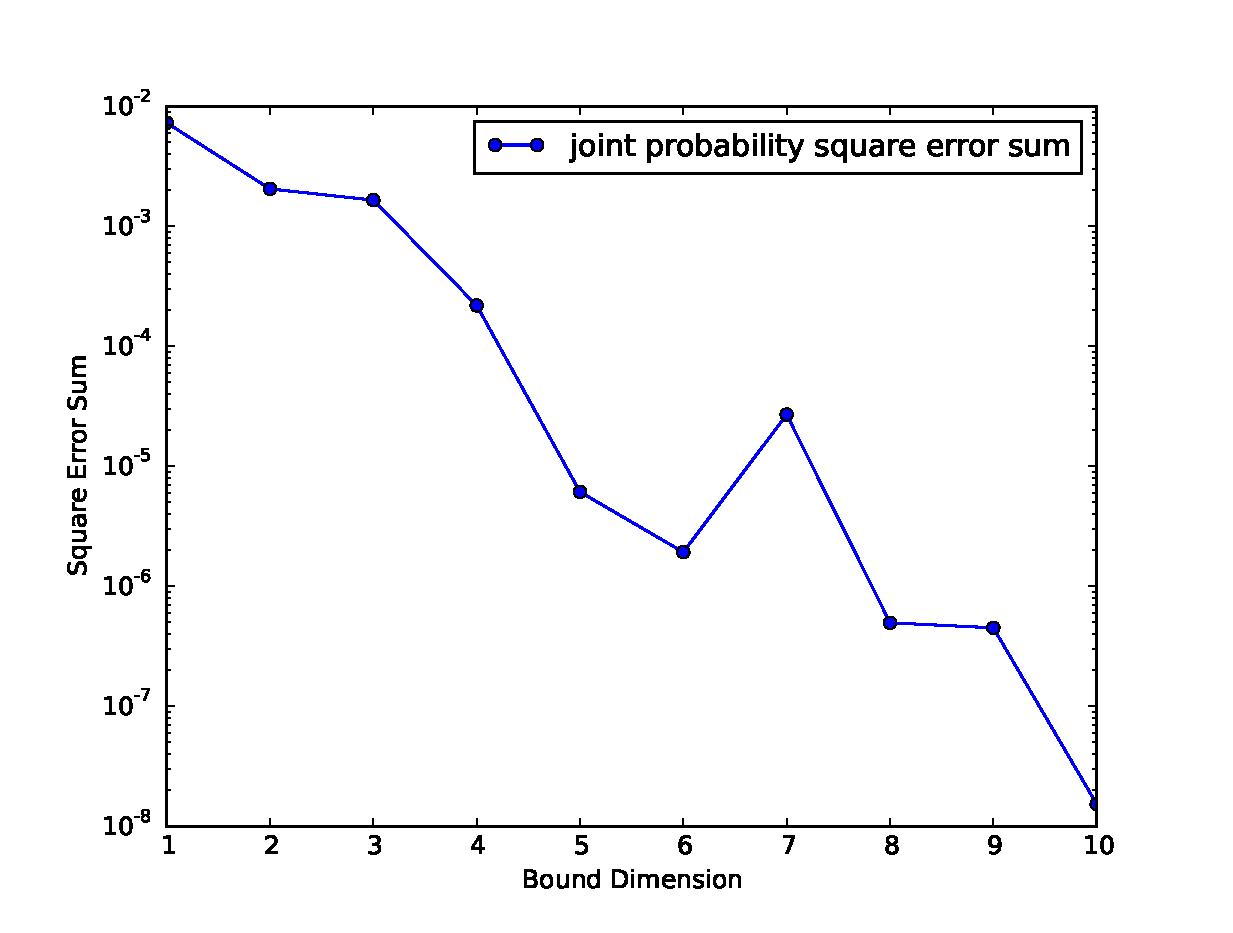
\includegraphics[scale=0.4]{Result_Fig/Radiating_Error_t100_s10_bd10_log.eps}}
\subfigure[MPS long chain]{
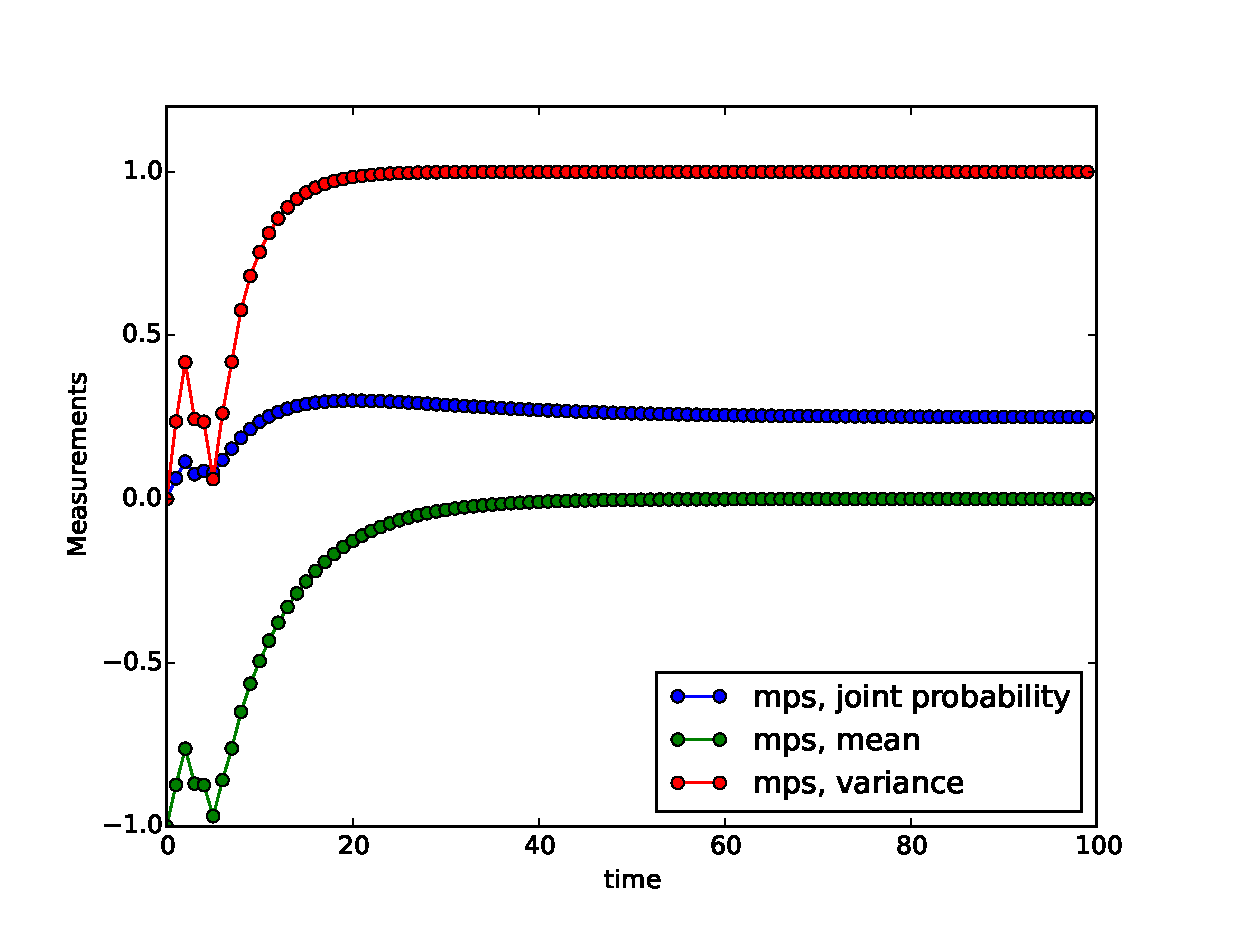
\includegraphics[scale=0.4]{Result_Fig/Radiating_MPS_t100_s30_bd10.eps}}\hfill
\subfigure[MPS with Different Bound Dimension]{
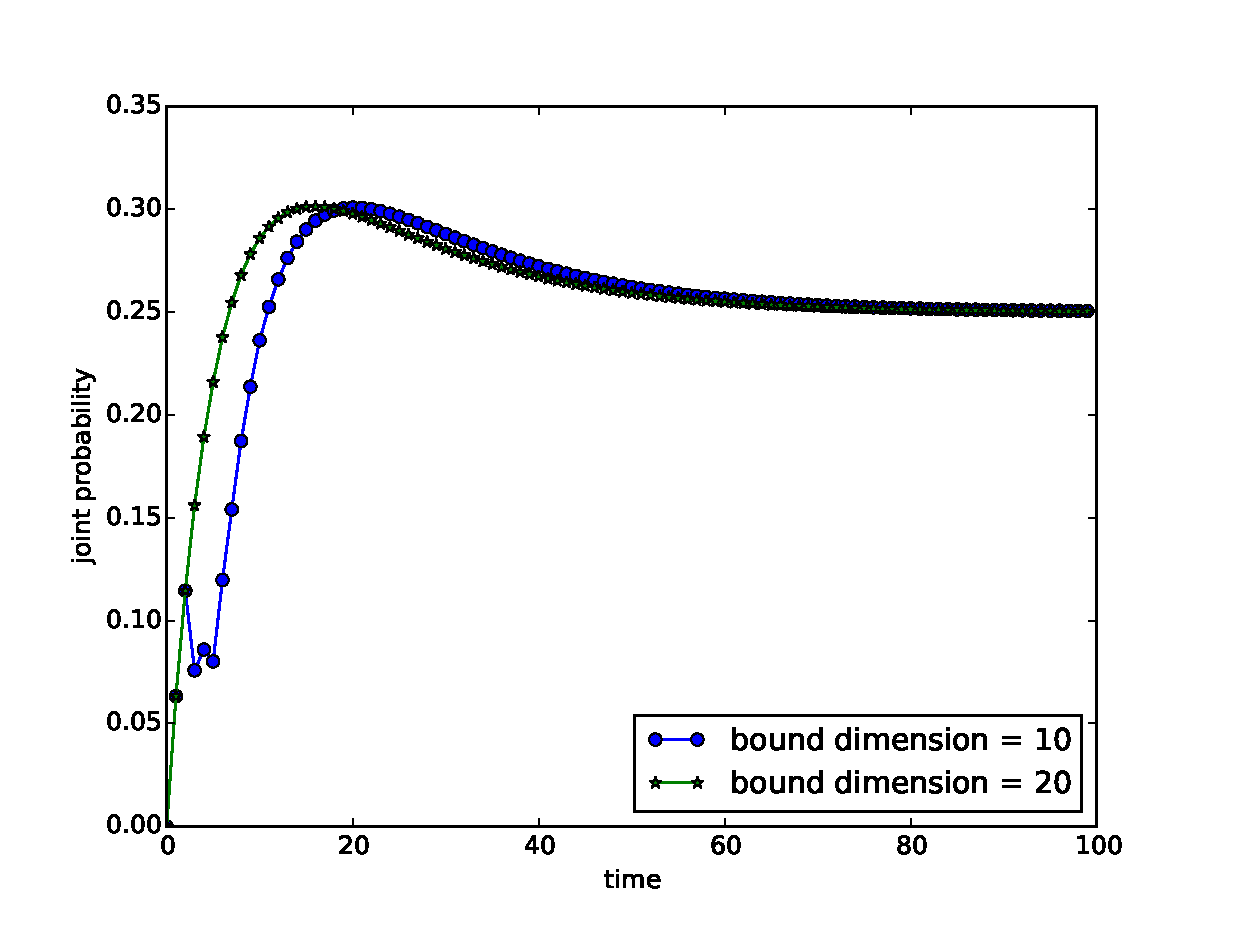
\includegraphics[scale=0.4]{Result_Fig/Radiating_MPS_t100_s30_bd10to20.eps}}
  % \end{minipage}\\[1em]
  \caption{Results of Radiating Boys Model.(a) gives the comparison of the joint probability, the mean value, and the variance between the MPS method and exact method. The chain size is 10, and the bound dimension $\chi$ is 10 in the MPS method. (b) shows the decay of square error sum with increasing bound dimensions. The error is computed between the approximation and exact methods with a fixed time step of 100. (c) is the result of the MPS method on a longer chain with size $L=30$. (d) compares the joint probability of the MPS method with two bound dimensions. The two curves converge in the long run.}
  \label{fig:Radiating_result}
\end{figure}

\subsection{ExponentialBoys Model}
Fig.\ref{fig:Exponential_result} is the result of the Exponential Boys Model. 
\begin{figure}[htbp]
\centering
\subfigure[Exact Model(Short Chain)]{
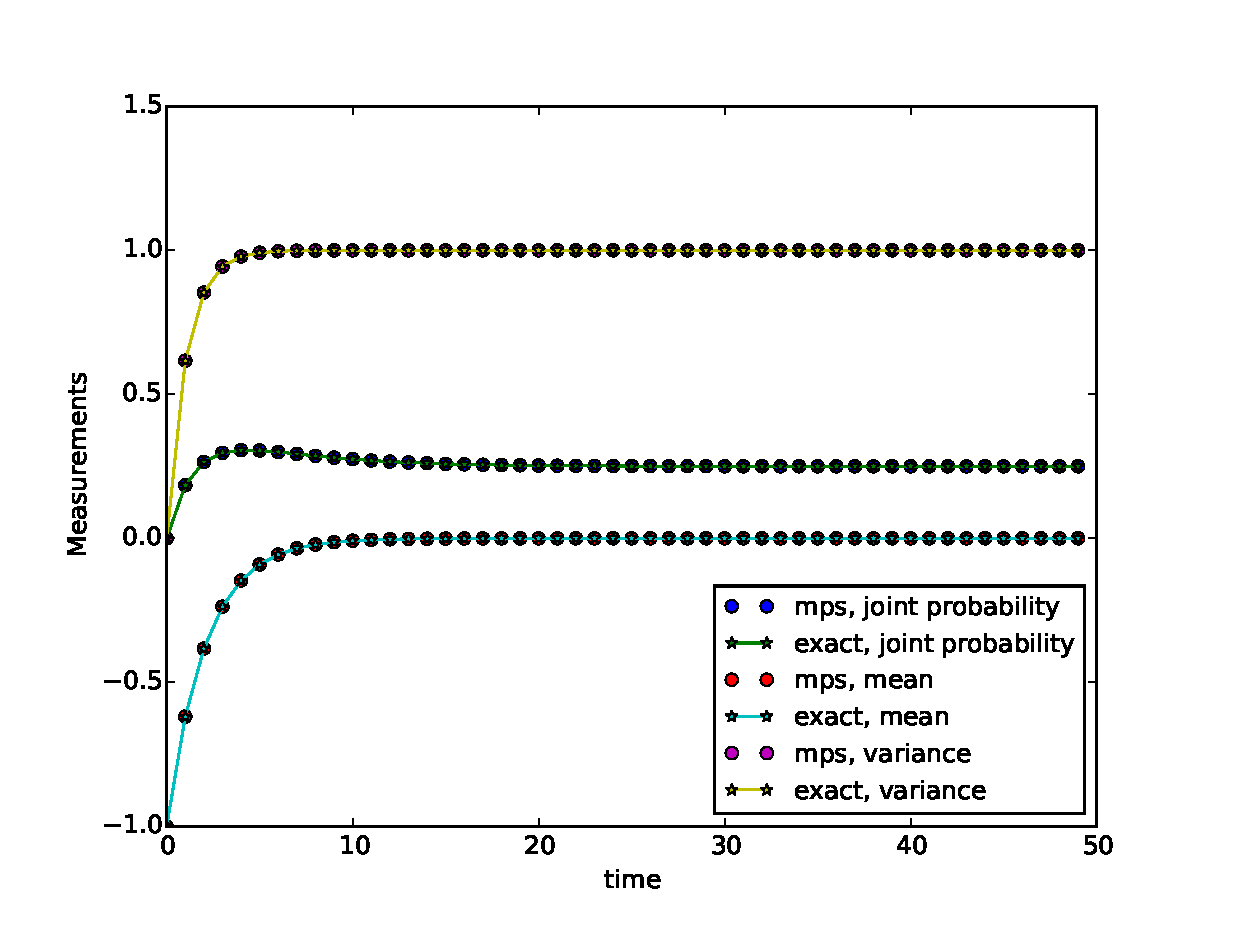
\includegraphics[scale=0.4]{Result_Fig/Exponential_Exact_t50_s10_bd10.eps}}\hfill
\subfigure[Error with Different Bound Dimension]{
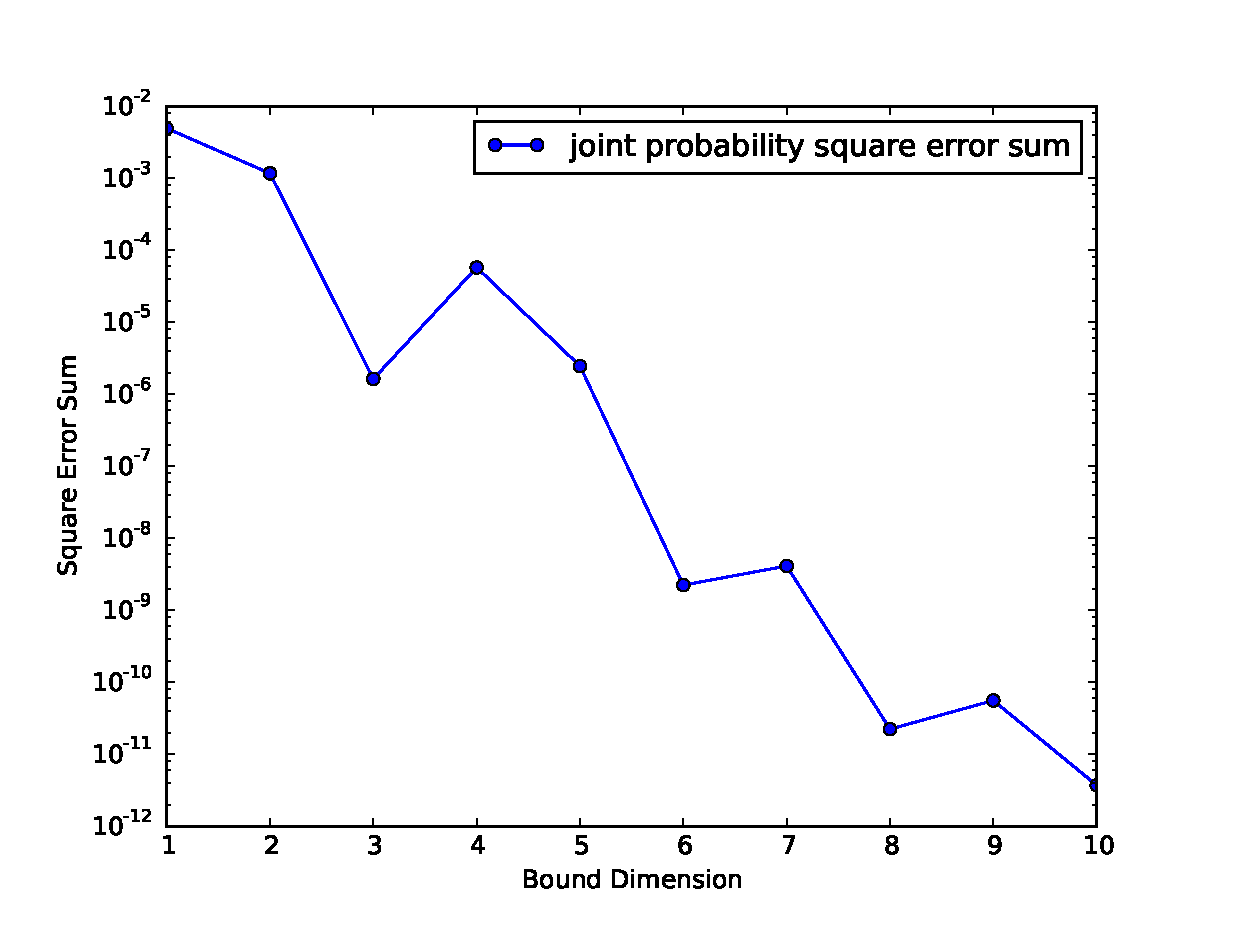
\includegraphics[scale=0.4]{Result_Fig/Exponential_Error_t100_s10_bd10_log.eps}}
\subfigure[MPS long chain]{
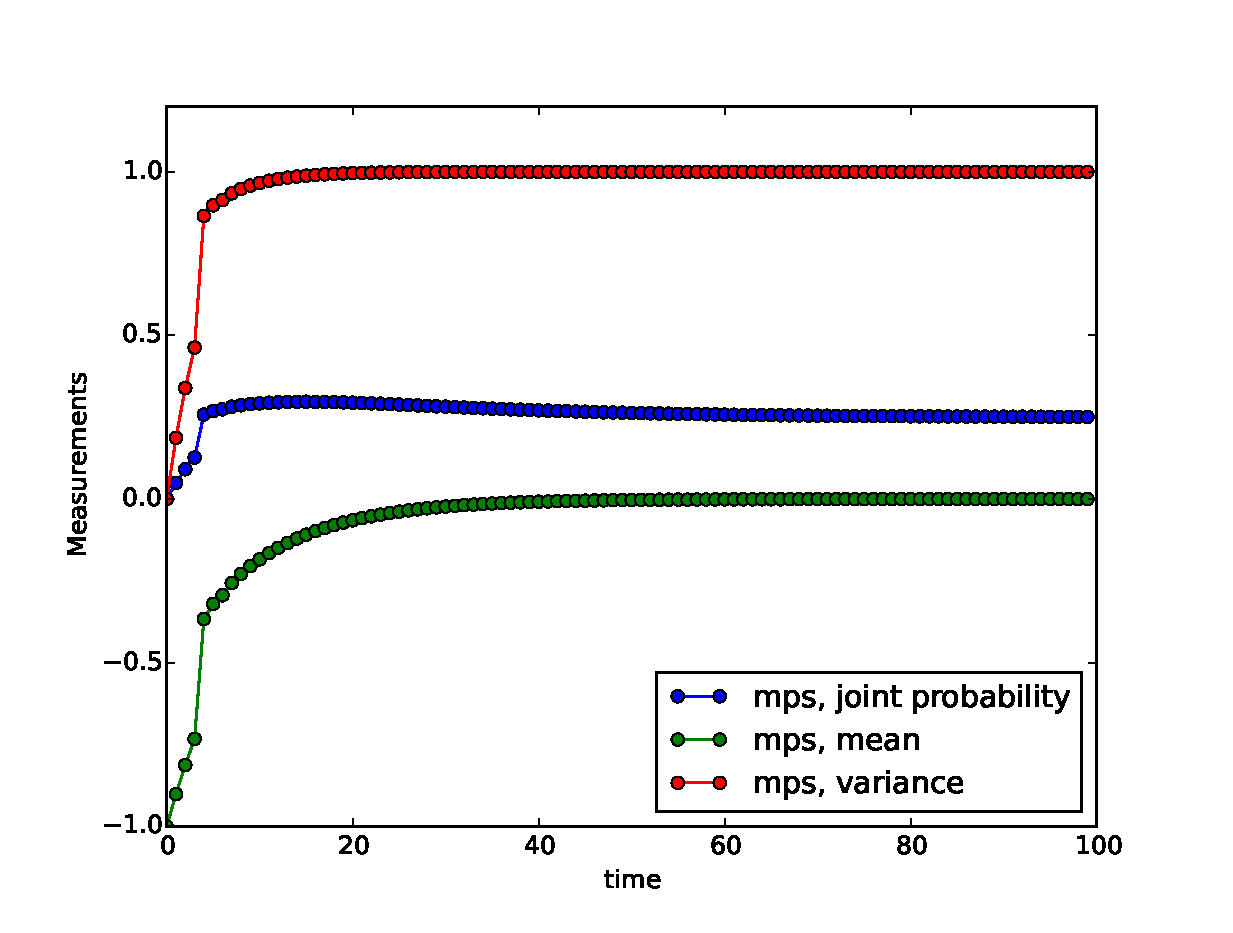
\includegraphics[scale=0.4]{Result_Fig/Exponential_MPS_t100_s40_bd10.eps}}\hfill
\subfigure[MPS with Different Bound Dimension]{
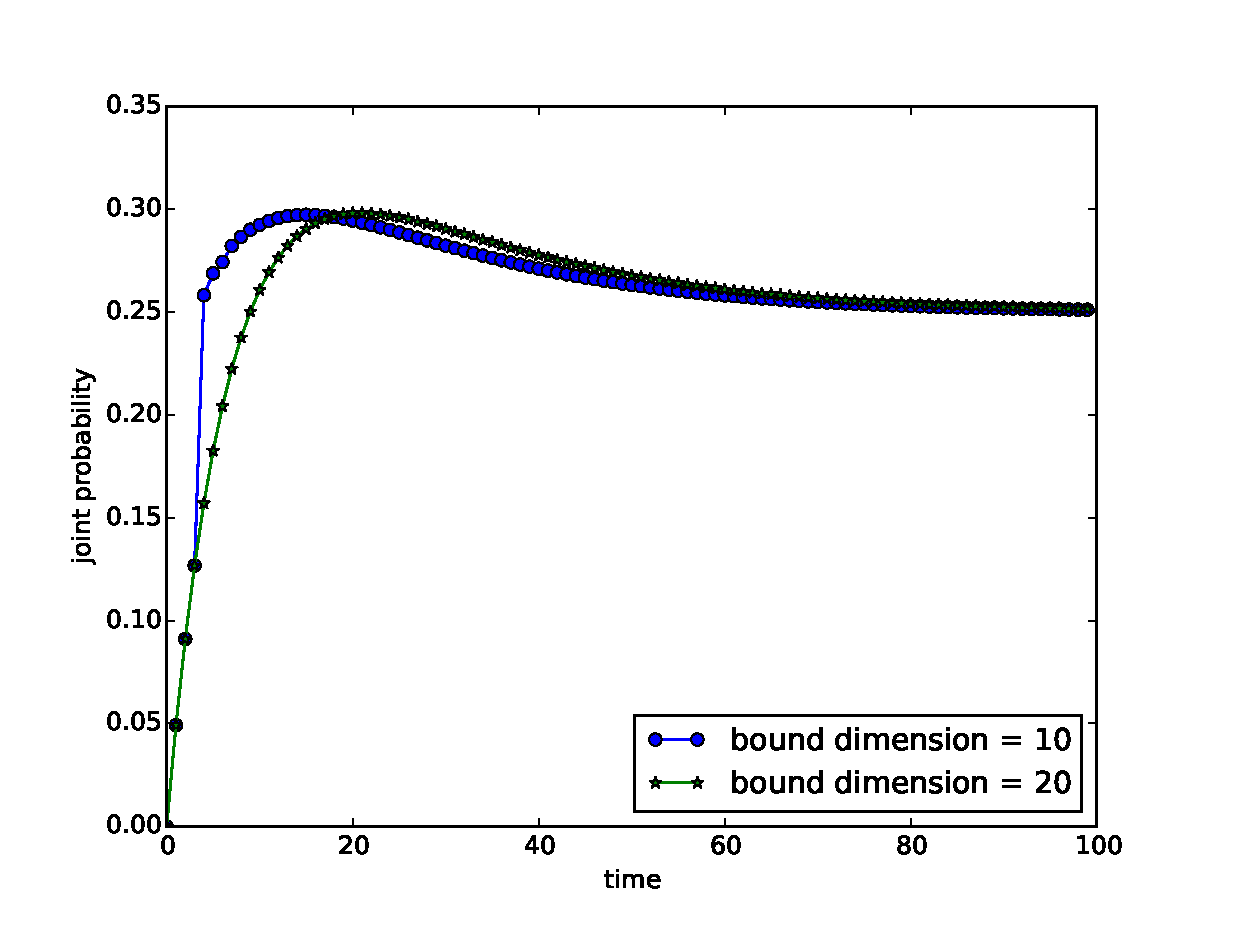
\includegraphics[scale=0.4]{Result_Fig/Exponential_MPS_t100_s40_bd10to20.eps}}
  % \end{minipage}\\[1em]
  \caption{Results of Exponential Boys Model.(a) gives the comparison of the joint probability, the mean value, and the variance between the MPS method and exact method. The chain size is 10, and the bound dimension $\chi$ is 10 in the MPS method. (b) shows the decay of square error sum with increasing bound dimensions. The error is computed between the approximation and exact methods with a fixed time step of 100. (c) is the result of the MPS method on a longer chain with the size $L=40$. (d) compares the joint probability of the MPS method with two bound dimensions. The two curves converge in the long run.}
  \label{fig:Exponential_result}
\end{figure}

\subsection{ProjectionBoys Model}
Fig.\ref{fig:Projection_result} is the result of the Projection Boys Model.
\begin{figure}[htbp]
\centering
\subfigure[Exact Model(Short Chain)]{
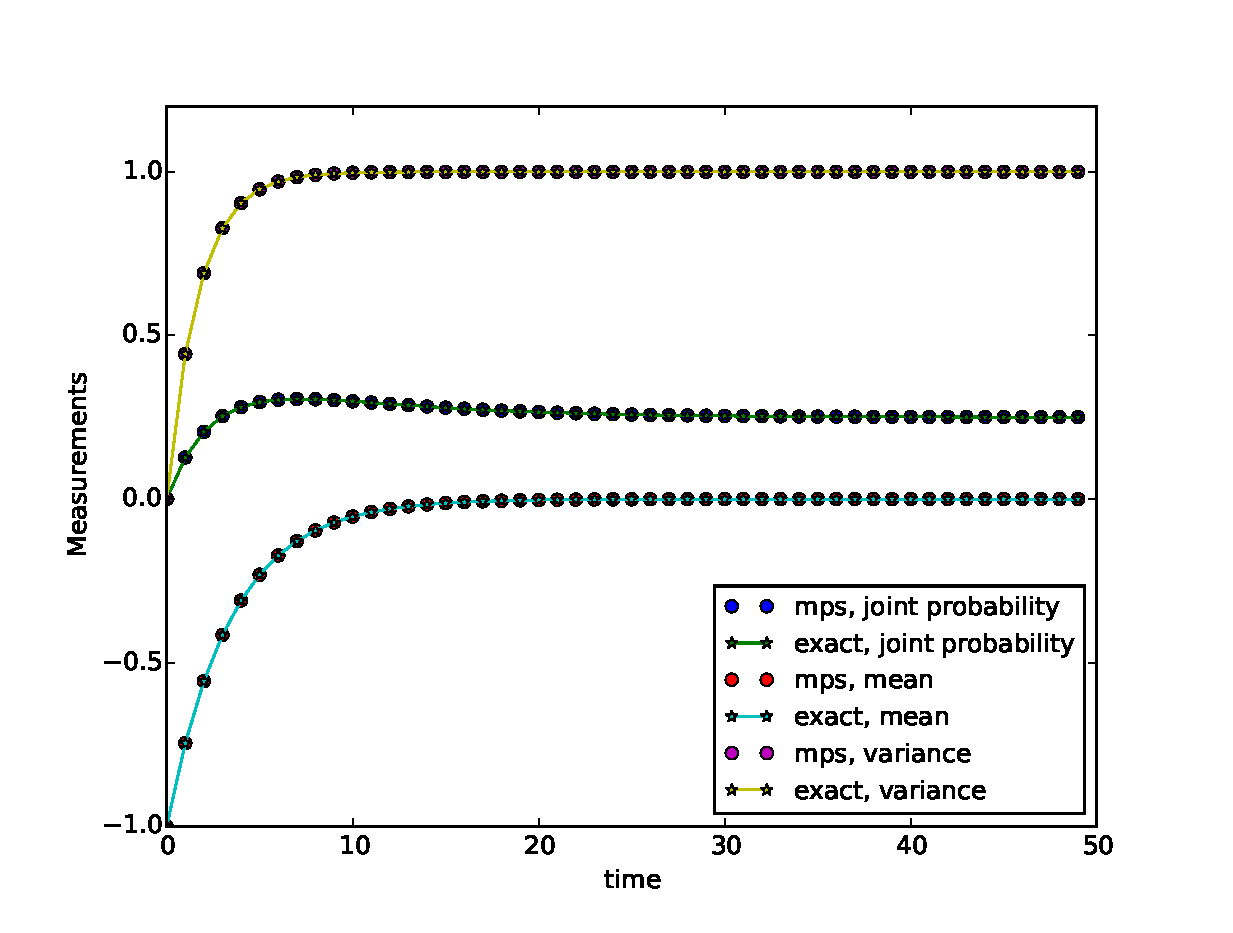
\includegraphics[scale=0.4]{Result_Fig/Projection_Exact_t50_s10_bd10.eps}}\hfill
\subfigure[Error with Different Bound Dimension]{
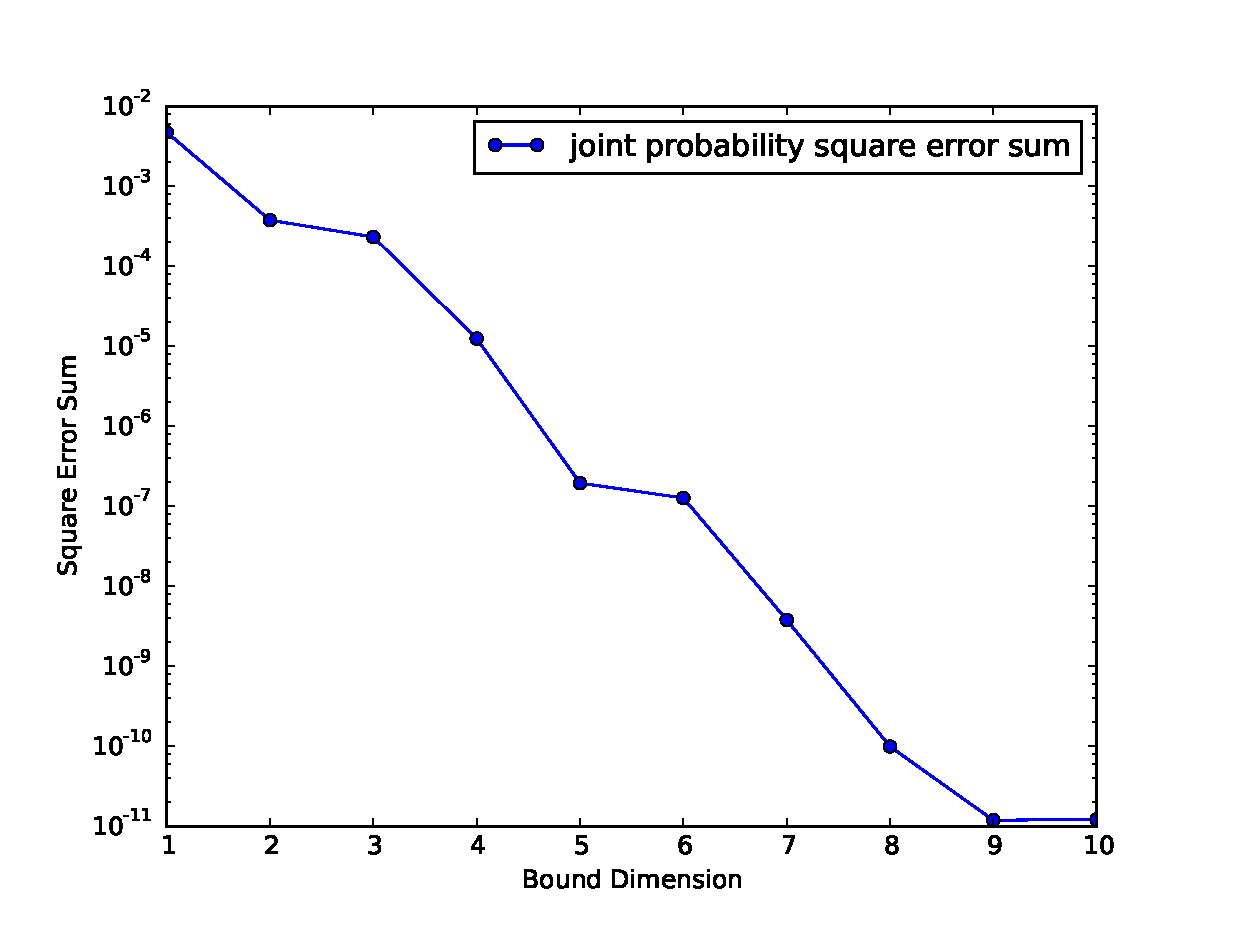
\includegraphics[scale=0.4]{Result_Fig/Projection_Error_t100_s10_bd10_log.eps}}
\subfigure[MPS long chain]{
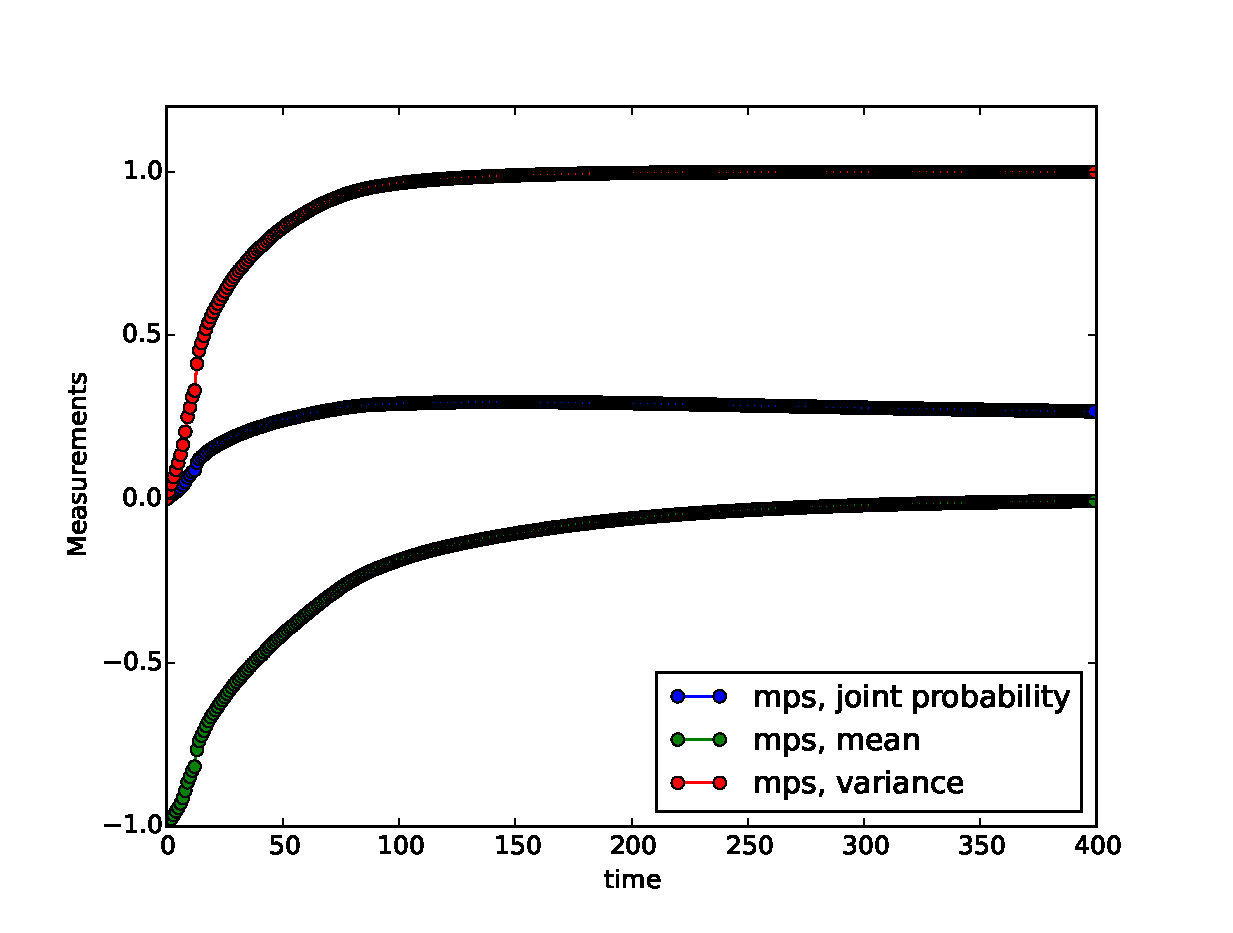
\includegraphics[scale=0.4]{Result_Fig/Projection_MPS_t400_s200_bd10.eps}}\hfill
\subfigure[MPS with Different Bound Dimension]{
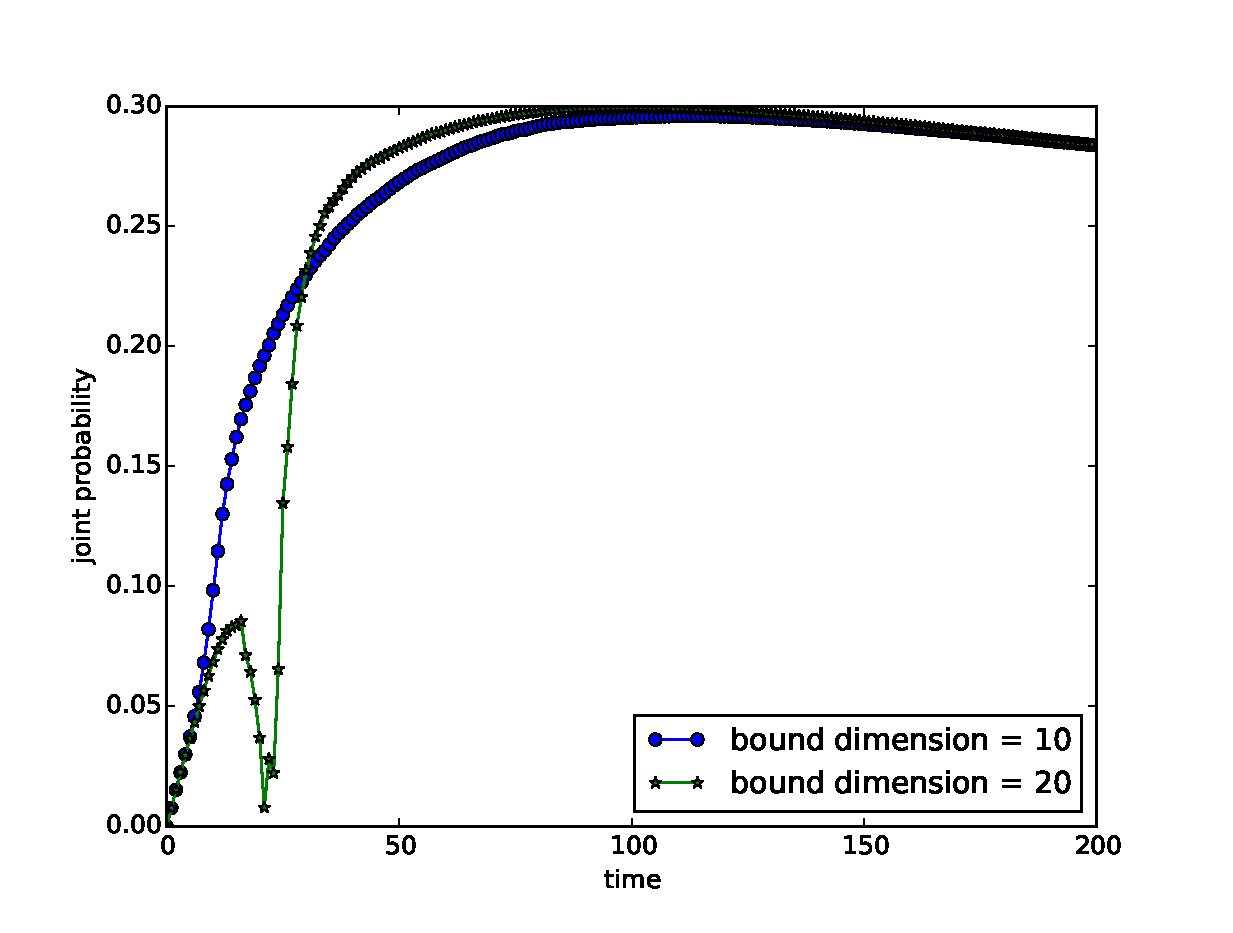
\includegraphics[scale=0.4]{Result_Fig/Projection_MPS_t200_s150_bd10to20.eps}}
  % \end{minipage}\\[1em]
  \caption{Results of Exponential Boys Model.(a) gives the comparison of the joint probability, the mean value, and the variance between the MPS method and exact method. The chain size is 10, and the bound dimension $\chi$ is 10 in the MPS method. (b) shows the decay of square error sum with  increasing bound dimensions. The error is computed between the approximation and exact methods with a fixed time step of 100. (c) is the result of the MPS method on a long chain with the size $L=150$. (d) compares the joint probability of the MPS method with two bound dimensions. The two curves converge in the long run.}
  \label{fig:Projection_result}
\end{figure}


\begin{thebibliography}{99}
\bibitem{white} S. R. White, {\it Physical Review Letters} {\bf 69}, 2863 (1992)
\bibitem{schollwock} Ulrich Schollwoeck, {\it Annals of Physics} {\bf 326}, 96 (2011)
\bibitem{cirac} Verstraete, F., and J. I. Cirac, (2004), arXiv:cond-mat/0407066v1
\bibitem{vidal}G. Evenbly, G. Vidal, {\it J Stat Phys} (2011) {\bf 145:} 891-918
\end{thebibliography}
\end{document}

